
%
\documentclass[12pt,journal,onecolumn]{IEEEtran}
%\documentclass[journal]{IEEEtran}



% *** GRAPHICS RELATED PACKAGES ***
%
\ifCLASSINFOpdf
  % \usepackage[pdftex]{graphicx}
  % declare the path(s) where your graphic files are
  % \graphicspath{{../pdf/}{../jpeg/}}
  % and their extensions so you won't have to specify these with
  % every instance of \includegraphics
  % \DeclareGraphicsExtensions{.pdf,.jpeg,.png}
\else
  % or other class option (dvipsone, dvipdf, if not using dvips). graphicx
  % will default to the driver specified in the system graphics.cfg if no
  % driver is specified.
  % \usepackage[dvips]{graphicx}
  % declare the path(s) where your graphic files are
  % \graphicspath{{../eps/}}
  % and their extensions so you won't have to specify these with
  % every instance of \includegraphics
  % \DeclareGraphicsExtensions{.eps}
\fi
% graphicx was written by David Carlisle and Sebastian Rahtz. It is
% required if you want graphics, photos, etc. graphicx.sty is already
% installed on most LaTeX systems. The latest version and documentation
% can be obtained at: 
% http://www.ctan.org/tex-archive/macros/latex/required/graphics/
% Another good source of documentation is "Using Imported Graphics in
% LaTeX2e" by Keith Reckdahl which can be found at:
% http://www.ctan.org/tex-archive/info/epslatex/
%
% latex, and pdflatex in dvi mode, support graphics in encapsulated
% postscript (.eps) format. pdflatex in pdf mode supports graphics
% in .pdf, .jpeg, .png and .mps (metapost) formats. Users should ensure
% that all non-photo figures use a vector format (.eps, .pdf, .mps) and
% not a bitmapped formats (.jpeg, .png). IEEE frowns on bitmapped formats
% which can result in "jaggedy"/blurry rendering of lines and letters as
% well as large increases in file sizes.
%
% You can find documentation about the pdfTeX application at:
% http://www.tug.org/applications/pdftex





% *** MATH PACKAGES ***
%
\usepackage[cmex10]{amsmath}

% correct bad hyphenation here
\hyphenation{op-tical net-works semi-conduc-tor}
\usepackage[utf8]{inputenc}
\usepackage[T1]{fontenc}
\usepackage[portuguese]{babel}
\usepackage{graphicx}
\usepackage{amsmath}
\usepackage{listings}
\usepackage{epstopdf}
\usepackage{array,url,kantlipsum}
\usepackage{afterpage}
\usepackage[space]{grffile}
\usepackage[framed,numbered,autolinebreaks,useliterate]{mcode}

\usepackage{caption}
\usepackage{subcaption}


\begin{document}

%
% paper title
% can use linebreaks \\ within to get better formatting as desired
% Do not put math or special symbols in the title.
\title{Relatório de Atividade - Redes Neurais Artificiais}

\author{David Clifte,~\IEEEmembership{Mestrando em Ciências da
Computação,~IFCE,}
}



% make the title area
\maketitle

% For peer review papers, you can put extra information on the cover
% page as needed:
% \ifCLASSOPTIONpeerreview
% \begin{center} \bfseries EDICS Category: 3-BBND \end{center}
% \fi
%
% For peerreview papers, this IEEEtran command inserts a page break and
% creates the second title. It will be ignored for other modes.
\IEEEpeerreviewmaketitle



\section{Introdução}
% The very first letter is a 2 line initial drop letter followed
% by the rest of the first word in caps.
% 
% form to use if the first word consists of a single letter:
% \IEEEPARstart{A}{demo} file is ....
% 
% form to use if you need the single drop letter followed by
% normal text (unknown if ever used by IEEE):
% \IEEEPARstart{A}{}demo file is ....
% 
% Some journals put the first two words in caps:
% \IEEEPARstart{T}{his demo} file is ....
% 
% Here we have the typical use of a "T" for an initial drop letter
% and "HIS" in caps to complete the first word.
\IEEEPARstart{N}{este} trabalho é apresentado o resultado da implementação do
Perceptron e do Adaline no Matlab. Inicialmente é apresentado o Classificador
Linear, base do funcionamento para o Perceptron e o Adaline e então é
apresentado os métodos e resultados do trabalho.

\hfill Setembro 21, 2014


\section{Classificador Linear}
Um classificador linear é capaz de dividir duas classes através de uma, reta,
plano ou hiperplano, dependendo do número de dimensões das características.
Isso é feito através do valor obtido da combinação linear das características.
Dependendo do valor escalar obtido dessa combinação é feita a decisão de qual 
classe pertence o vetor de características ou vetor de entradas.

Uma combinação linear é o resultado do produto de cada termo de um vetor por uma
constante e os resultados são então somados. Como exemplo temos a combinação
linear de $a \times \overrightarrow{x} + b \times \overrightarrow{y}$ onde a e
b são constantes e $\overrightarrow{x}$ e $\overrightarrow{y}$ vetores
pertencentes ao mesmo espaço vetorial.

Podemos ainda generalizar combinação linear como um produto de matrizes.
Dada uma matriz \textbf{A} onde cada coluna é um vetor que será combinado.
Seja \textbf{C} uma matriz com os coeficientes. A combinação linear pode ser
representada como:
\newline 

$A \times B 
=
\begin{bmatrix}
 a_{11} & a_{1..} & a_{1n} \\ 
 a_{..1} & a_{....} & a_{....} \\ 
 a_{m1} & a_{m..} & a_{mn} \\ 
\end{bmatrix}
\times
\begin{bmatrix}
 c_{1} \\ c_{..} \\ c_{n}\\ 
\end{bmatrix}
\newline
=
c_{1} \times \begin{bmatrix} a_{11} \\ a_{..1} \\ a_{m1}\\  \end{bmatrix}
+
c_{..} \times \begin{bmatrix} a_{1..} \\ a_{....} \\ a_{m..}\\  \end{bmatrix}
+
...
+
c_{n} \times \begin{bmatrix} a_{1n} \\ a_{....} \\ a_{mn}\\  \end{bmatrix}$
\newline
A saída obtida por um classificador linear pode ser obtida através da seguinte
equação.
$y = f(\overrightarrow{w}\cdot\overrightarrow{x}) = f\left(\sum_j w_j x_j\right)$,
onde $\overrightarrow{w}$ é um vetor com valores reais que representam os
coeficientes da combinação linear, geralmente chamado de pesos do
classificador, $\overrightarrow{x}$ o vetor de características que será
avaliado e y o valor escalar resultante da combinação linear.

% needed in second column of first page if using \IEEEpubid
%\IEEEpubidadjcol
\section{Perceptron}
Um perceptron é um classificador linear. Se dois conjuntos de pontos podem ser
separados linearmente pode-se utilizar o perceptron para fazer a classificação,
para tanto é necessário ajustar os pesos para as sinapses. 

O perceptron tem duas limitações. Primeiro, os valores de saída do perceptron
podem assumir somente dois valores (Verdadeiro ou Falso). Segundo, perceptrons
somente podem classificar grupos de vetores linearmente separados, como dito
anteriormente. Para realizar a classificação de mais de uma classe é
necessário um número maior de perceptrons, entretanto ainda sim as classes
devem ser linearmente separáveis.Na figura \ref{fig:perceptron} temos a
representação de um perceptron.
De forma geral, nos neurônios artificiais os seguintes elementos estão
envolvidos:

Conjunto de sinapses (W): Ligações entre neurônios. Cada ligação possui um valor
(peso), que representa a sua força: os estímulos de entrada são multiplicados
pelos repectivos pesos de cada ligação, podendo gerar um sinal tanto positivo
(exitatório) quanto negativo (inibitório).

Combinador Linear(): Executa o somatório dos sinais produzidos pelo produto
entre os pesos sinápticos e as entradas fornecidas ao neurônio. Em outras
palavras, é o integrador dos sinais que chegam ao neurônio.

Como pode ser observado o vetor de entrada \textit{in(t)} possui os
seguintes valores (x1, x2, ..., xn). (w1, w2, ..., wn) representam o respectivo
valor do peso do vetor de entrada.


\begin{figure}[h]
	\centering
	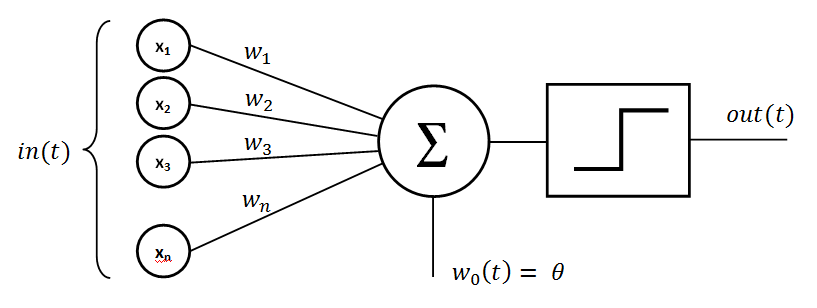
\includegraphics[width=10cm]{images/perceptron.png}
	\caption{Modelo de um perceptron.}
	\label{fig:perceptron}
\end{figure}



\subsection{Treinamento}
O algoritmo de aprendizagem é um método adaptativo em que o perceptron faz os
ajustes necessários nos pesos para se adequar a saída desejada. Isso é feito
através da apresentação repetida das $n$ amostras de treinamento e da correção
dos pesos para cada amostra.
A correção é feita até que o erro das amostras de treinamentos seja minimizado.
O vetor de entrada é combinado com os pesos e o resultado, um escalar, é
avaliado por uma função degral. 

Durante a fase de treinamento o perceptron é acionado por um vetor de entradas
$\overrightarrow{x}(n)$ onde $n$ representa a amostra apresentada ao perceptron.
O sinal de saída $y(n)$ é calculado pelo perceptron e então comparado com a
saída desejada $d(n)$. Com isso o erro $e(n)$ é para o perceptron é produzido.
\begin{align}
	e(n)=d(n)-y(n)
\end{align}
O $e(n)$ é utilizado para fazer a correção dos pesos utilizados pelo perceptron.
Isso é feito atravéz da minimização da função de custo, definida em função do
erro como:
\begin{align}
	\epsilon(n)=\frac{1}{2}e^2(n)
\end{align}

O ajuste no peso é feito atravéz da regra delta, definida por Widrow-Hoff. Na
regra é realizado o ajuste dos pesos sinápticos  $w(i)$, onde $i$ representa o
peso do neurônio assiciado a entrada $x(i)$.
\begin{align}
		 \Delta W = \eta e(n) x(n)
\end{align}

O ajuste feito em um peso sináptico de um perceptron é proporcional ao produto
do sinal de erro pelo sinal de entrada da sinapse em questão.
De acordo com o valor do peso da conexão podemos verificar se ela é do tipo
inibitória ou excitatória. Caso o valor do peso seja maior que zero a conexão é
dita excitatória, caso contrário, inibitória.

Afim de simplificar os cálculos, é comum fazer a adição do bias ao vetor de
pesos e ao vetor de entrada. Essa versão adicionada de bias é comumente chamada
de versão extendida da entrada e dos pesos.\newline Tendo como base a figura
\ref{fig:perceptron} temos:
$x$ é o vetor de entrada, $w$ é o vetor de pesos, $\theta$ é o bias e y é a
saída calculada em função dos pesos e da entrada.
A saída é calculada usando a seguinte equação:

\begin{align}
	y=f(\sum_{j=1}^{n} x_j w_j + \theta)
\end{align}
 
Onde $n$ é o número de entradas,  $f(\overrightarrow{w}^T \cdot \overrightarrow{x})$ é a função de
ativação aplicada na saída calculada, no perceptron é uma função degral. Como
dito anteriormente é comum adicionar o bias ao vetor de entrada e ao vetor de pesos. O valor adicionado ao
bias de entrada neste trabalho foi 1. Com a versão extendida da entrada e dos
pesos o calculo realizado é apenas um produto de matrizes $y=
\overrightarrow{w}^T \cdot \overrightarrow{x}$.


\subsection{Operador AND, OR e NOT}
A base de dados foi criada para os operadores AND, OR e NOT de forma
programática. Dado um conjunto de dados gerados aleatóriamente, os valores das
saídas foram calculados de acordo com o operador desejado. Os detalhes para a
contrução da base podem ser verificados na sessão \ref{subsec:geraBase}
localizada no Apêndice.








\subsubsection{Operador AND}
Nesta sessão são exibido os resultados obtidos para o operador lógico AND.
A tabela verdade do operador AND pode ser visualizada na
tabela \ref{tab:verd_AND};
Os dados utilizados no treinamento estão expressos na figura \ref{fig:AND_dados}.


\begin{table}[!htbp]
\caption{Tabela verdade do operador AND}
\label{tab:verd_AND}
\centering
	\begin{tabular}{| c | c | c |}
		\hline
		 $x_1$  & $x_2$ 	& $y$ \\ \hline
		 0      & 0 		& 0 \\ \hline
		 0 		& 1 		& 0 \\ \hline
		 1 		& 0 		& 0 \\ \hline
		 1 		& 1 		& 1 \\
		\hline
	\end{tabular}
\end{table}


\begin{figure}[!htbp]
	\centering
	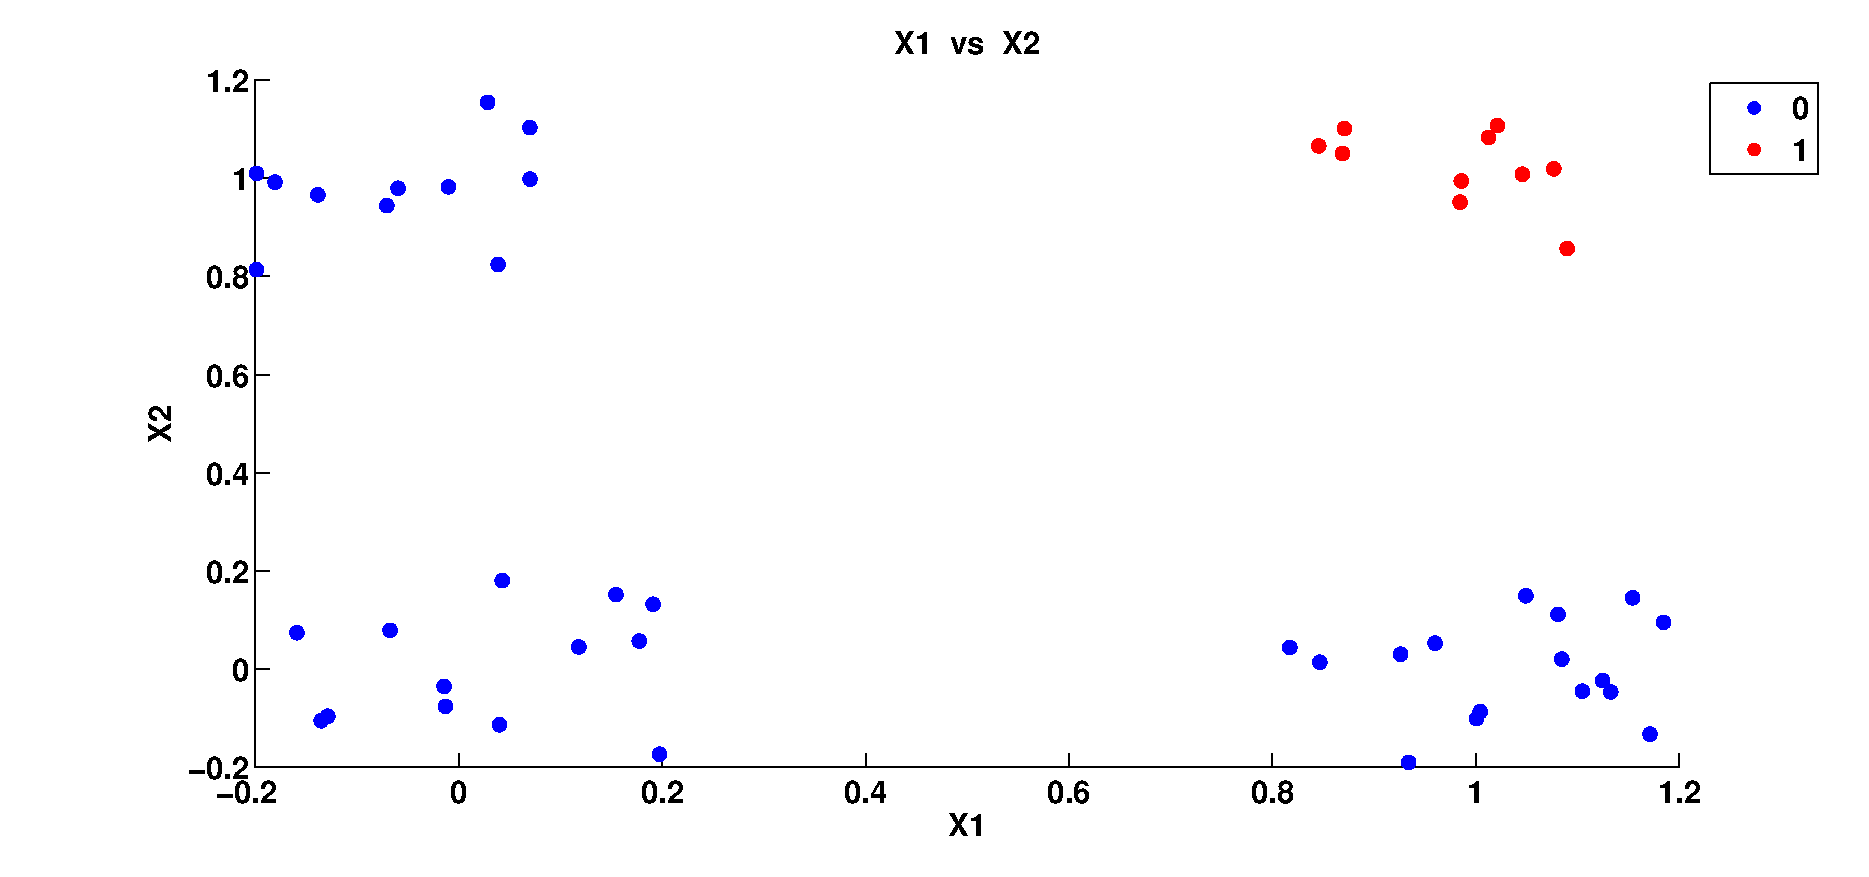
\includegraphics[width=10cm, trim = 3cm 1cm 3cm 1cm, clip=true
	]{eps/and/ANDDesired.eps}
	\caption{Dados utilizados no treinamento. Em vermelho os valores onde o
	operador AND tem como resultado o valor 1 em função dos valores de X1 e X2}
	\label{fig:AND_dados}
\end{figure} 

A seguir, figura \ref{fig:AND_err}, é exibido o erro quadrático médio obtido
durante o treinamento.
É exibido também o erro global, percentual de acerto da época durante o
treinamento usando as amostras de treinamento.

\begin{figure}[!htbp]
	\centering
	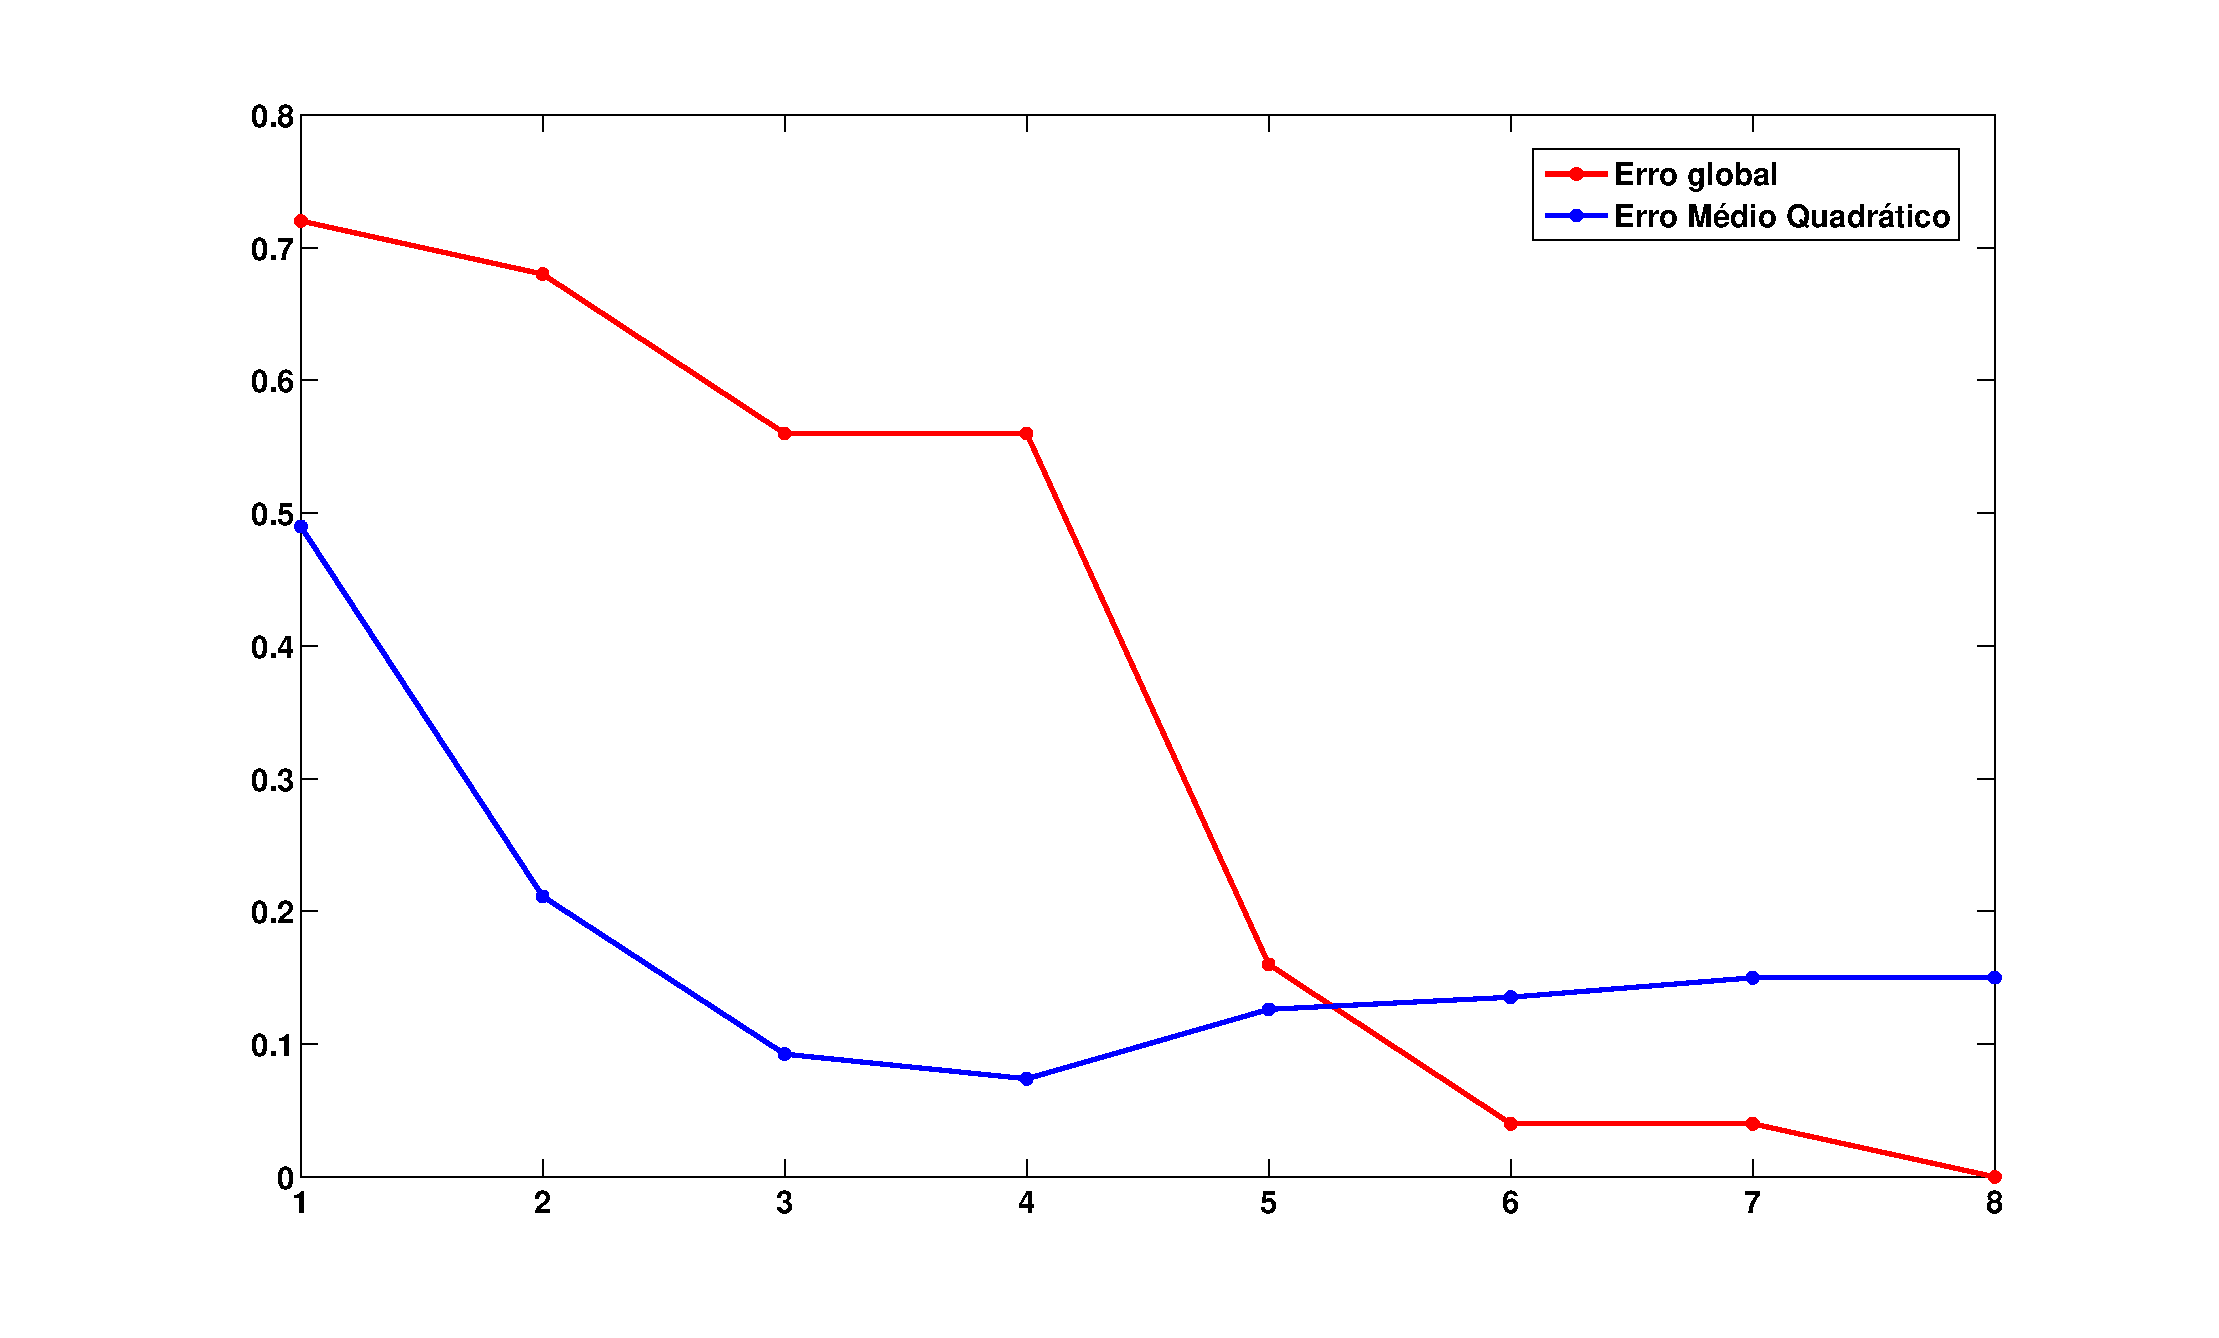
\includegraphics[width=10cm, trim = 3cm 1cm 3cm 1cm, clip=true
	]{eps/and/andErr.eps}
	\caption{Erro obtido durante cada época do treinamento do operador AND.}
	\label{fig:AND_err}
\end{figure} 

Após o treinamento é possível calcular a região de decisão traçada pelo
perceptron, figura \ref{fig:andReg}.

\begin{figure}[!htbp]
	\centering
	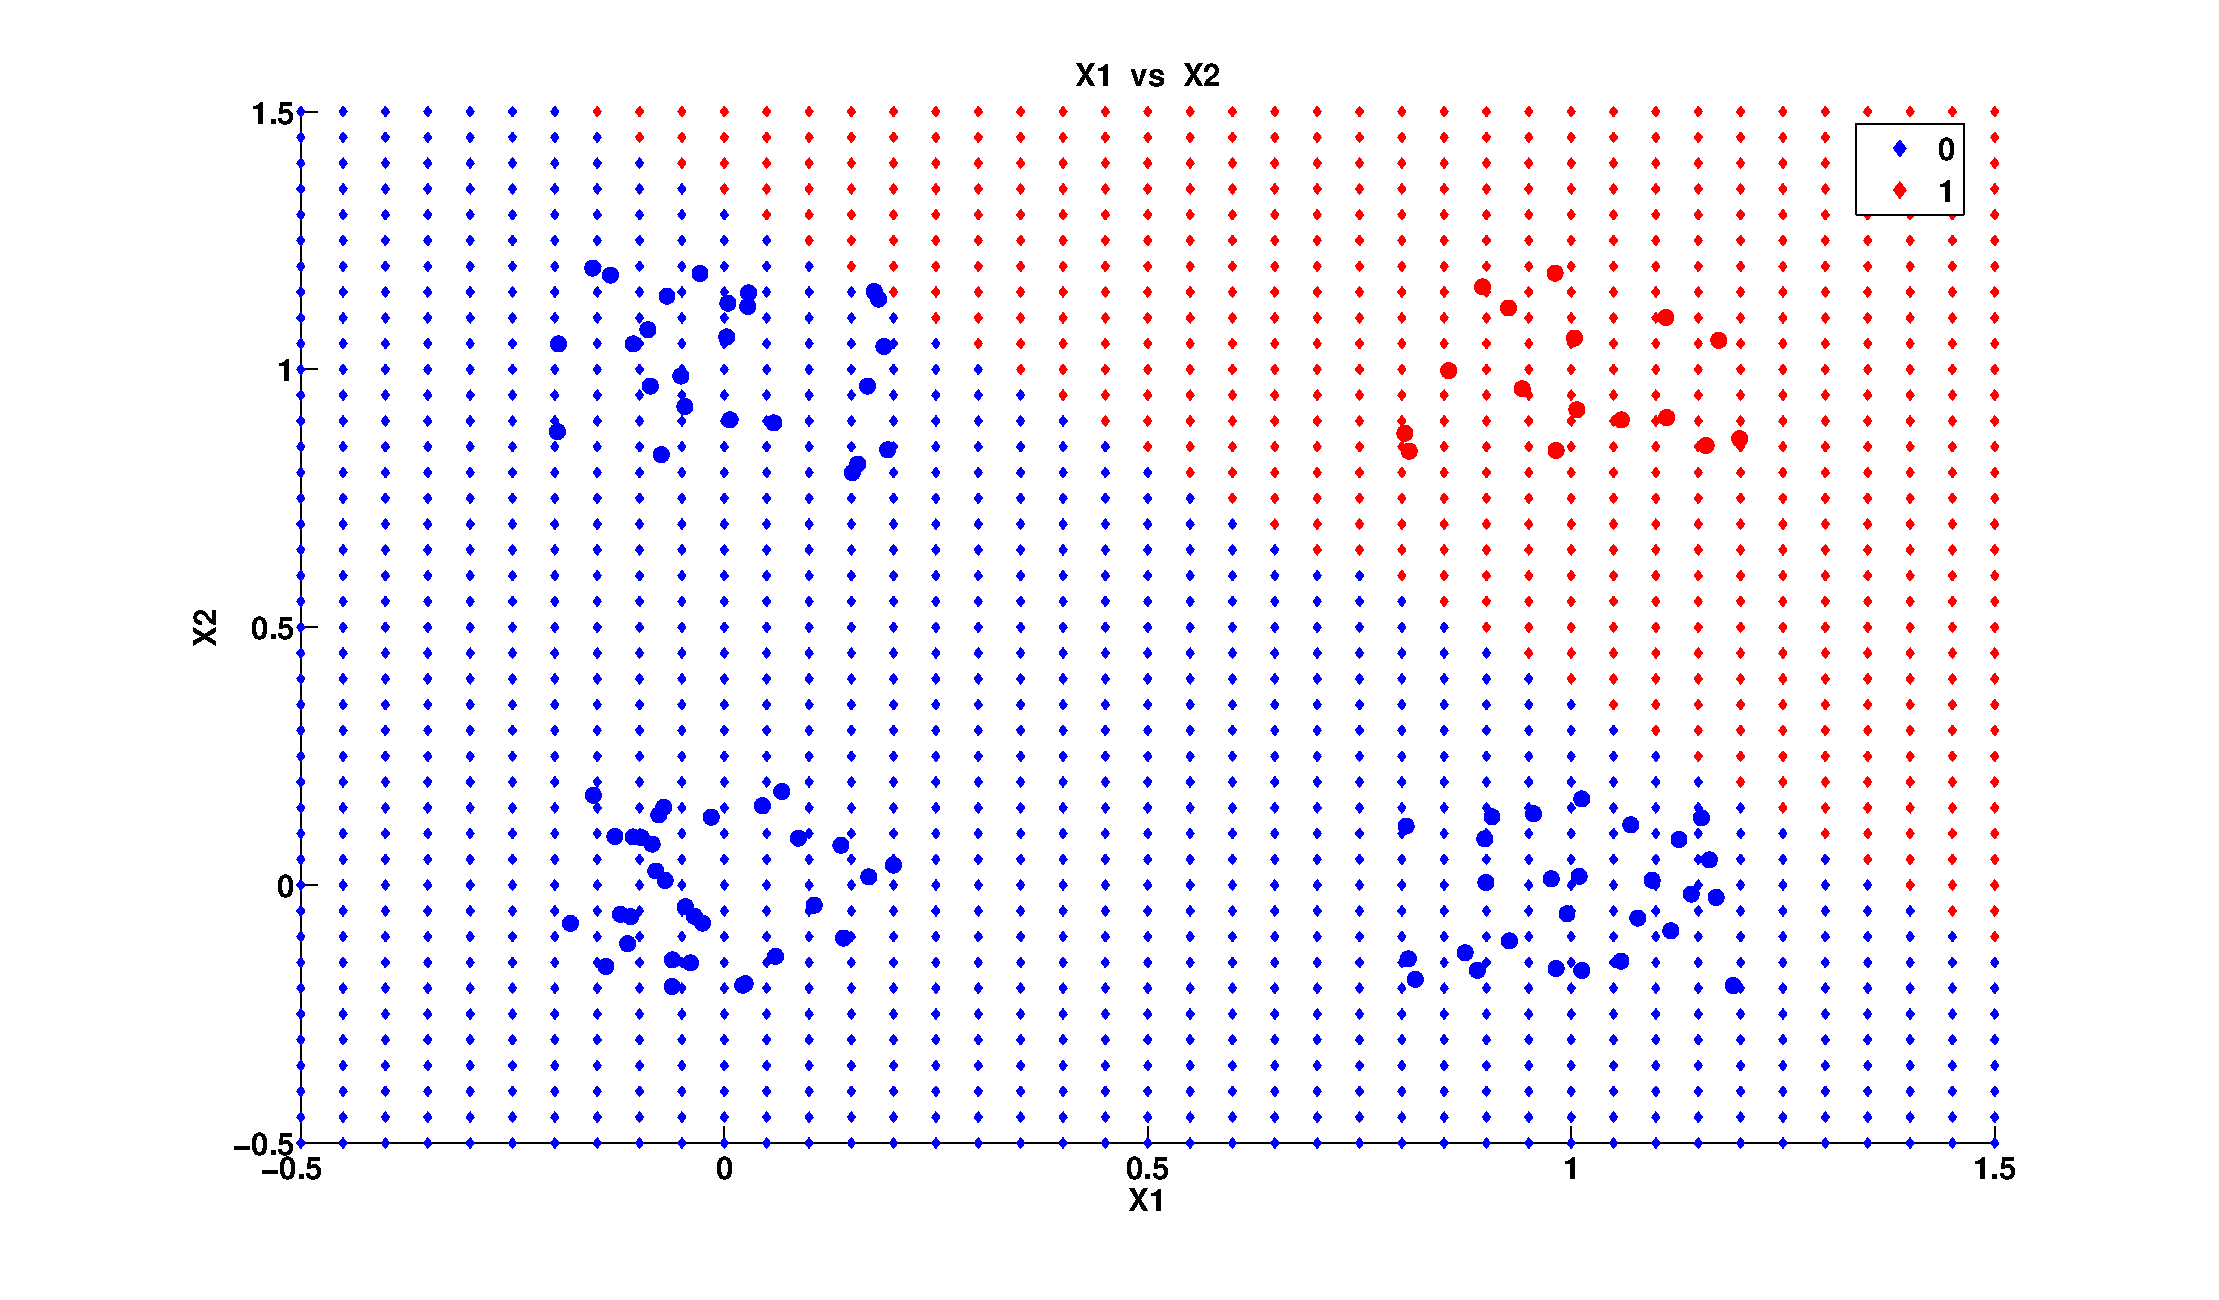
\includegraphics[width=10cm, trim = 3cm 1cm 3cm 1cm, clip=true
	]{eps/and/ANDRegiao.eps}
	\caption{Região de decisão calculada para a porta AND após o treinamento. O
	fundo pontilhado indica a região de decisão. Em vermelho a região em que as
	amostras são classificadas como 1. Os pontos de raio maior são os dados de
	treinamento.}
	\label{fig:andReg}
\end{figure} 

\subsubsection{Operador OR}
Nesta sessão são exibido os resultados obtidos para o operador lógico OR.
A tabela verdade do operador OR pode ser visualizada na
tabela \ref{tab:verd_OR};
Os dados utilizados no treinamento estão expressos na figura \ref{fig:OR_dados}.

\begin{table}[!htbp]
\caption{Tabela verdade do operador OR}
\label{tab:verd_OR}
\centering
	\begin{tabular}{| c | c | c |}
		\hline
		 $x_1$  & $x_2$ 	& $y$ \\ \hline
		 0      & 0 		& 0 \\ \hline
		 0 		& 1 		& 1 \\ \hline
		 1 		& 0 		& 1 \\ \hline
		 1 		& 1 		& 1 \\
		\hline
	\end{tabular}
\end{table}



\begin{figure}[!htbp]
	\centering
	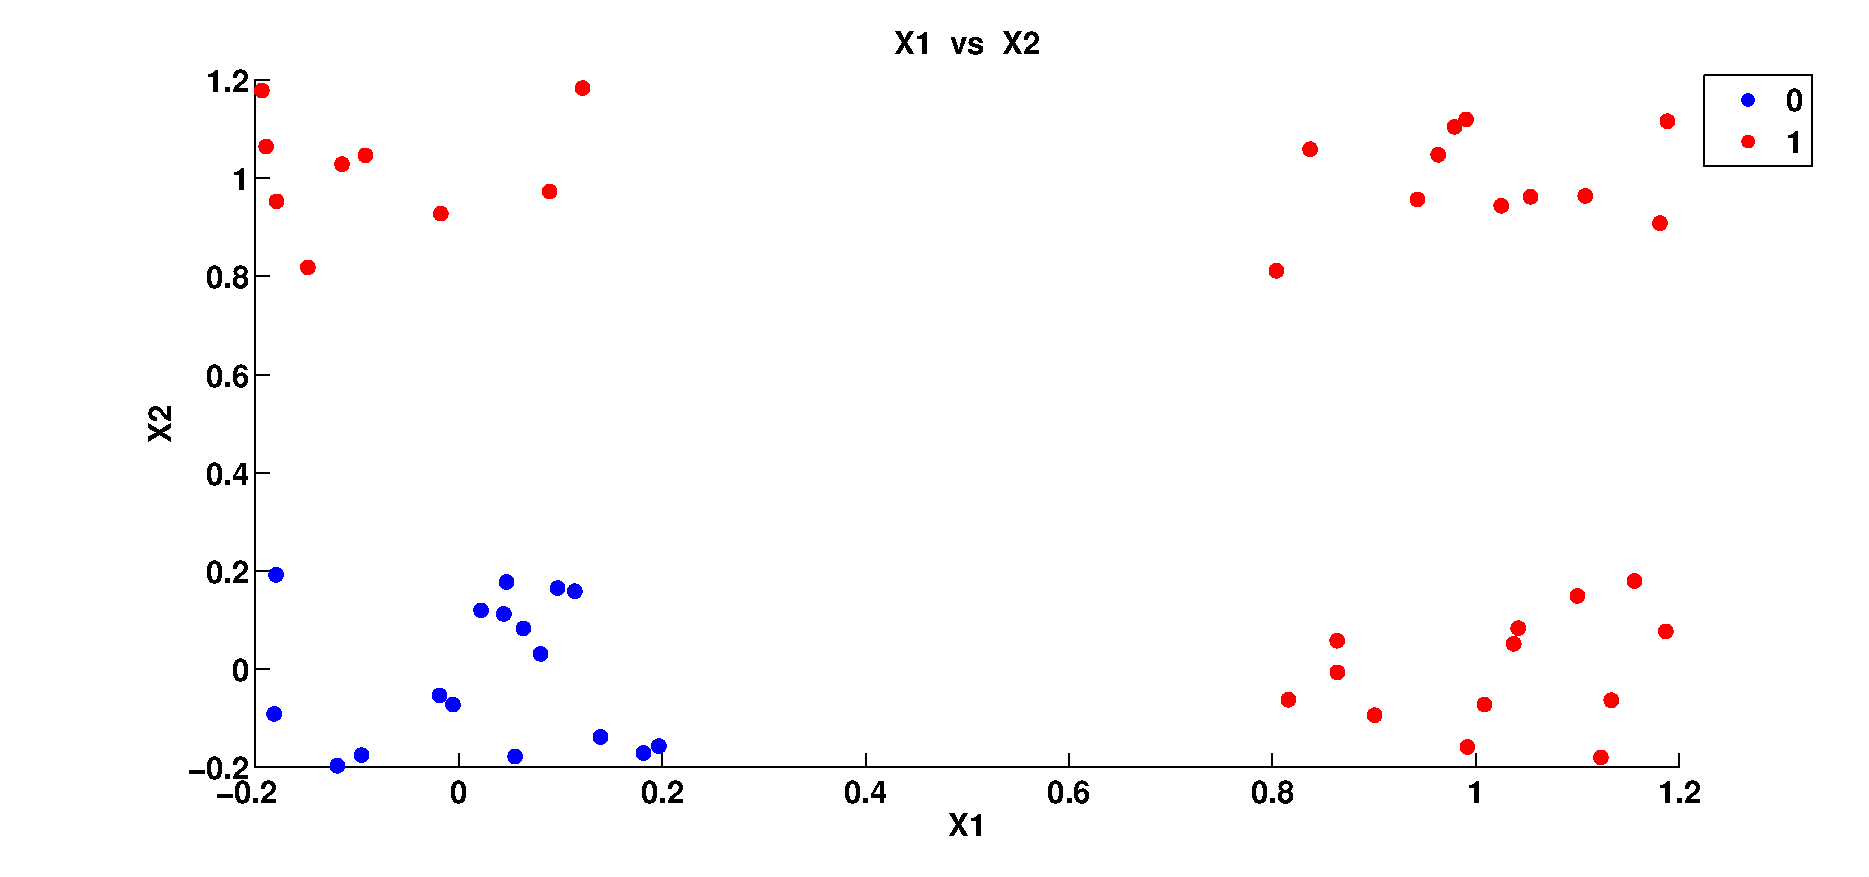
\includegraphics[width=10cm, trim = 3cm 1cm 3cm 1cm, clip=true
	]{eps/or/ORDesired.eps}
	\caption{Dados utilizados no treinamento. Em vermelho os valores onde o
	operador OR tem como resultado o valor 1 em função dos valores de X1 e X2}
	\label{fig:OR_dados}
\end{figure} 

A seguir, figura \ref{fig:OR_err} é exibido o erro quadrático médio obtido durante o
treinamento.
É exibido também o erro global, percentual de acerto da época durante o
treinamento usando as amostras de treinamento.
\begin{figure}[!htbp]
	\centering
	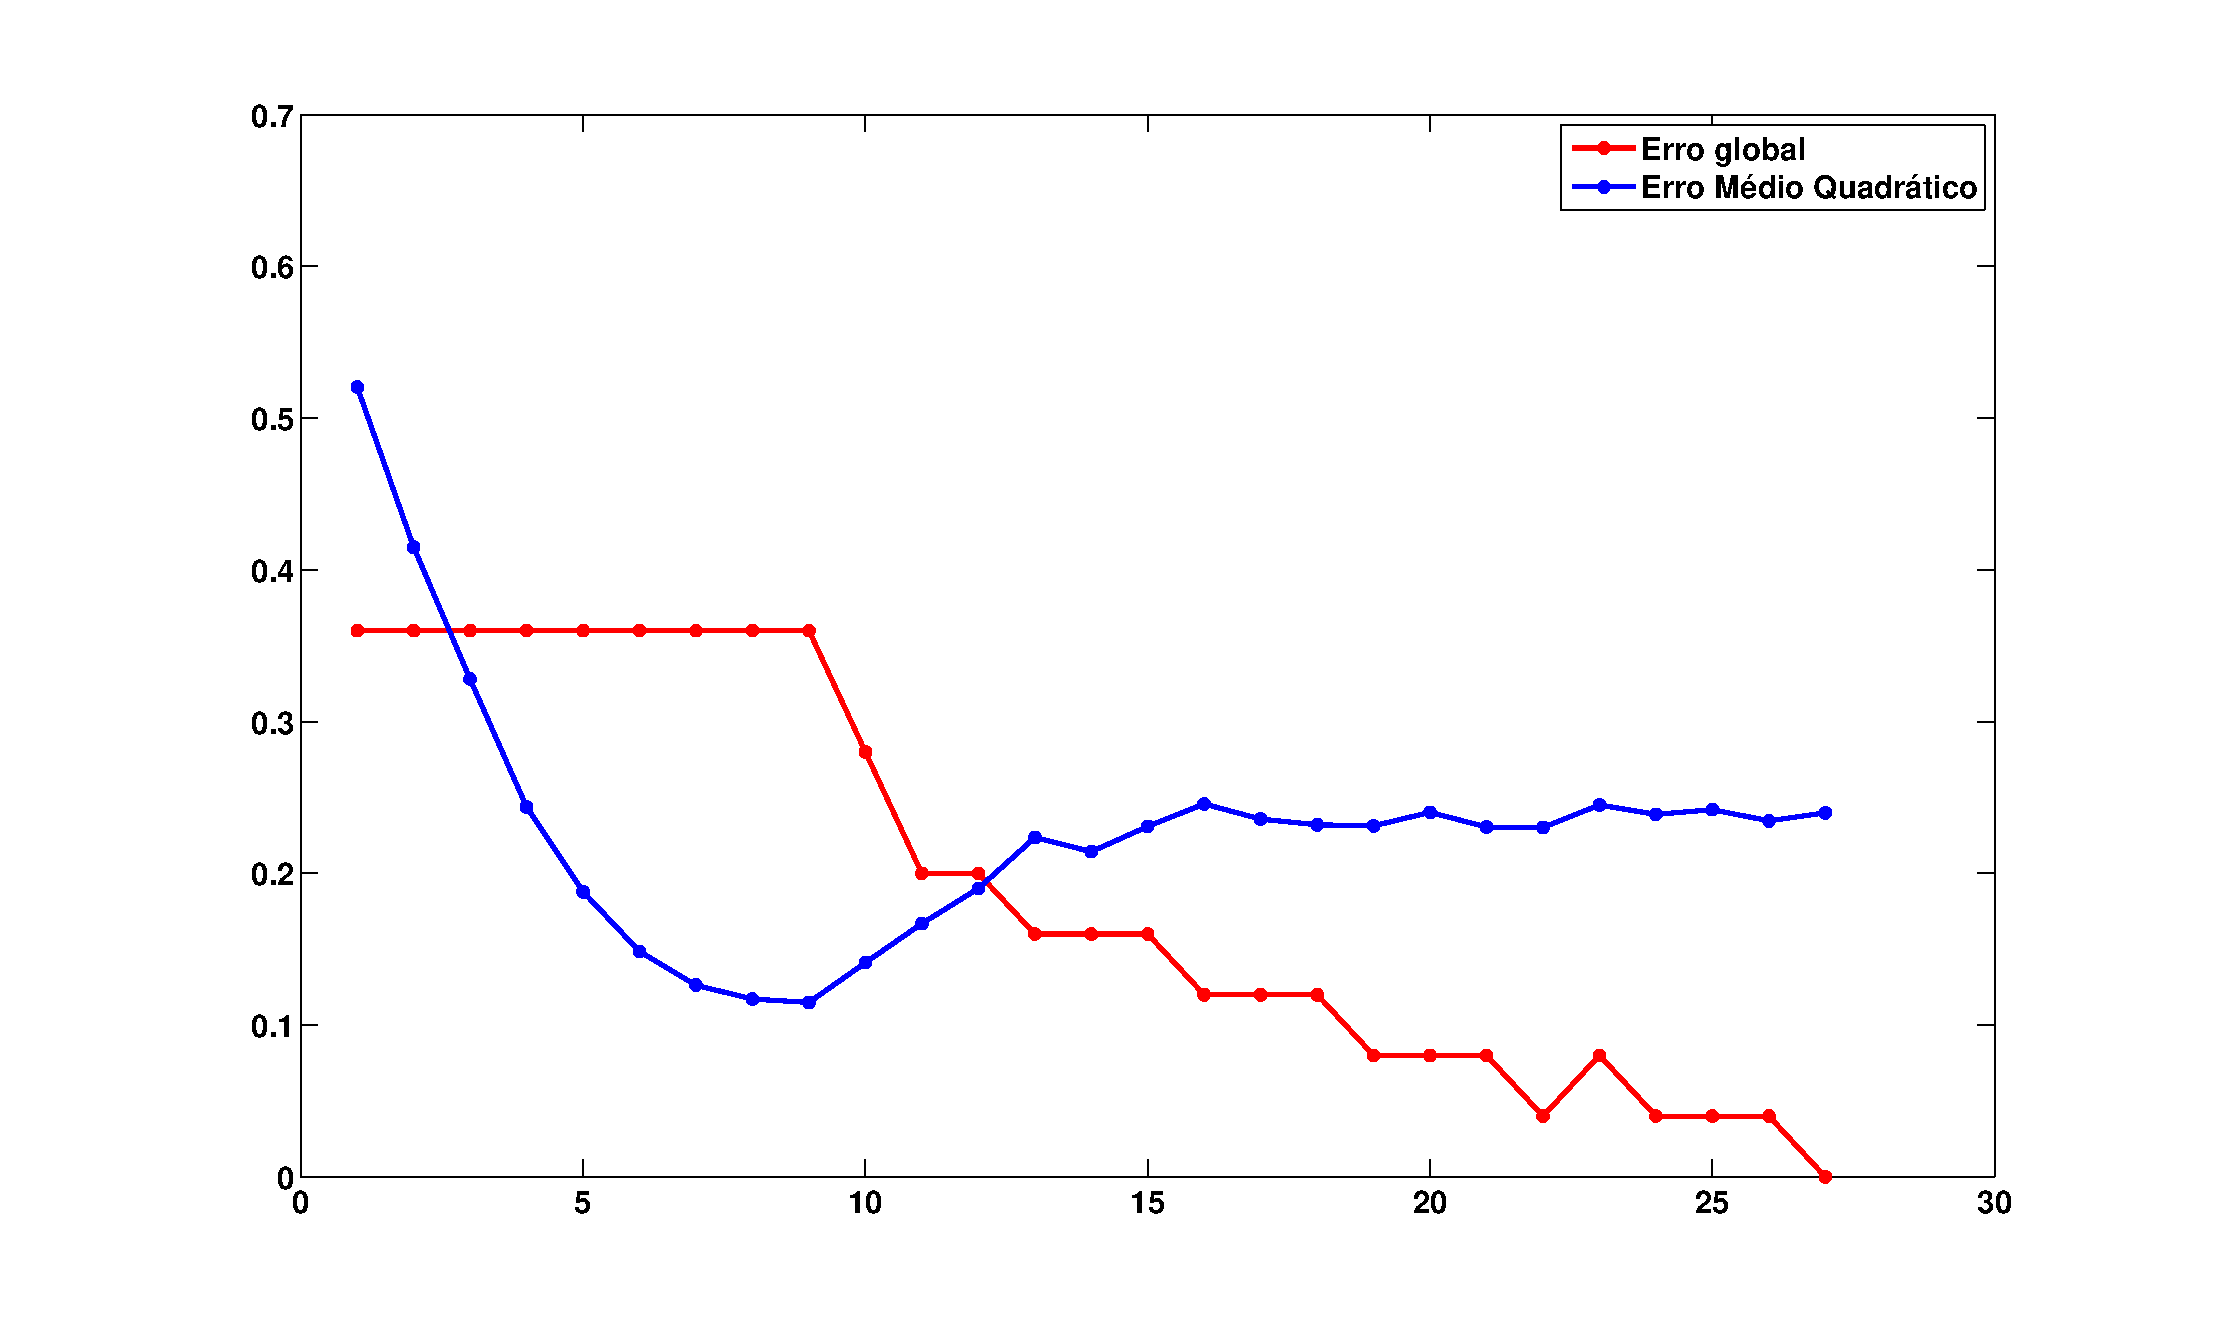
\includegraphics[width=10cm, trim = 3cm 1cm 3cm 1cm, clip=true
	]{eps/or/orErr.eps}
	\caption{Erro obtido durante cada época do treinamento}
	\label{fig:OR_err}
\end{figure} 

Após o treinamento é possível calcular a região de decisão traçada pelo
perceptron, figura \ref{fig:ORReg}.

\begin{figure}[!htbp]
	\centering
	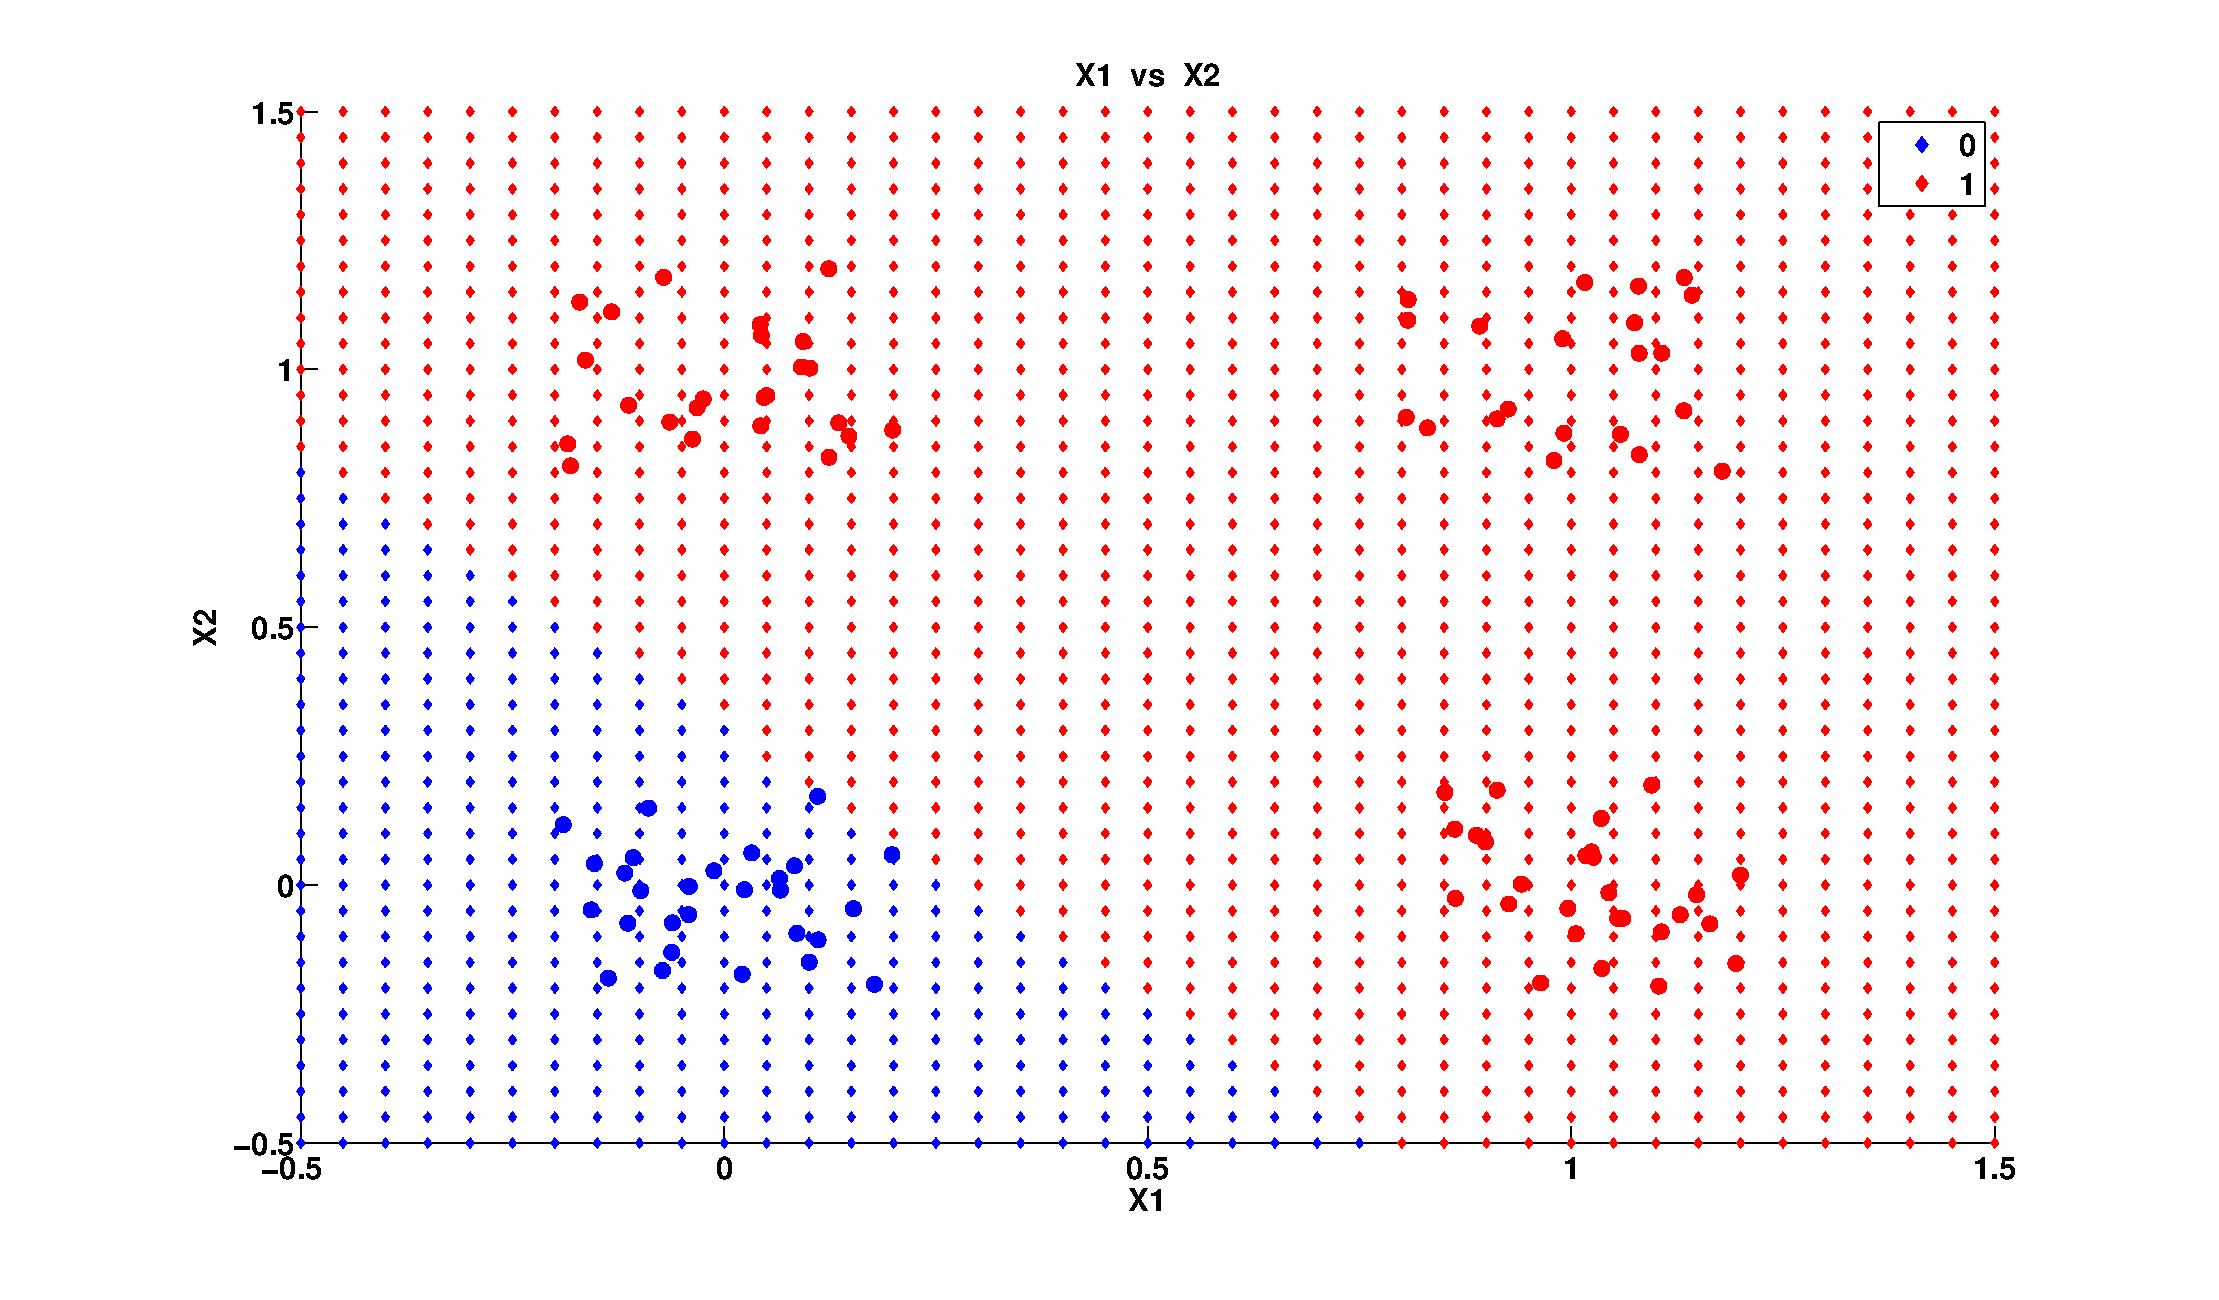
\includegraphics[width=10cm, trim = 3cm 1cm 3cm 1cm, clip=true
	]{eps/or/ORRegiao.eps}
	\caption{Região de decisão calculada para a porta OR após o treinamento. O
	fundo pontilhado indica a região de decisão. Em vermelho a região em que as
	amostras são classificadas como 1. Os pontos de raio maior são os dados de
	treinamento.}
	\label{fig:ORReg}
\end{figure} 


\subsubsection{Operador NOT}
Nesta sessão são exibido os resultados obtidos para o operador lógico NOT.
A tabela verdade do operador NOT pode ser visualizada na
tabela \ref{tab:verd_NOT};
Os dados utilizados no treinamento estão expressos na figura \ref{fig:NOT_dados}.

\begin{table}[!htbp]
\caption{Tabela verdade do operador NOT}
\label{tab:verd_NOT}
\centering
	\begin{tabular}{| c | c |}
		\hline
		 $x$ 	& $y$ \\ \hline
		 0      & 1 \\ \hline
		 1 		& 0 \\ \hline

		\hline
	\end{tabular}
\end{table}


\begin{figure}[!htbp]
	\centering
	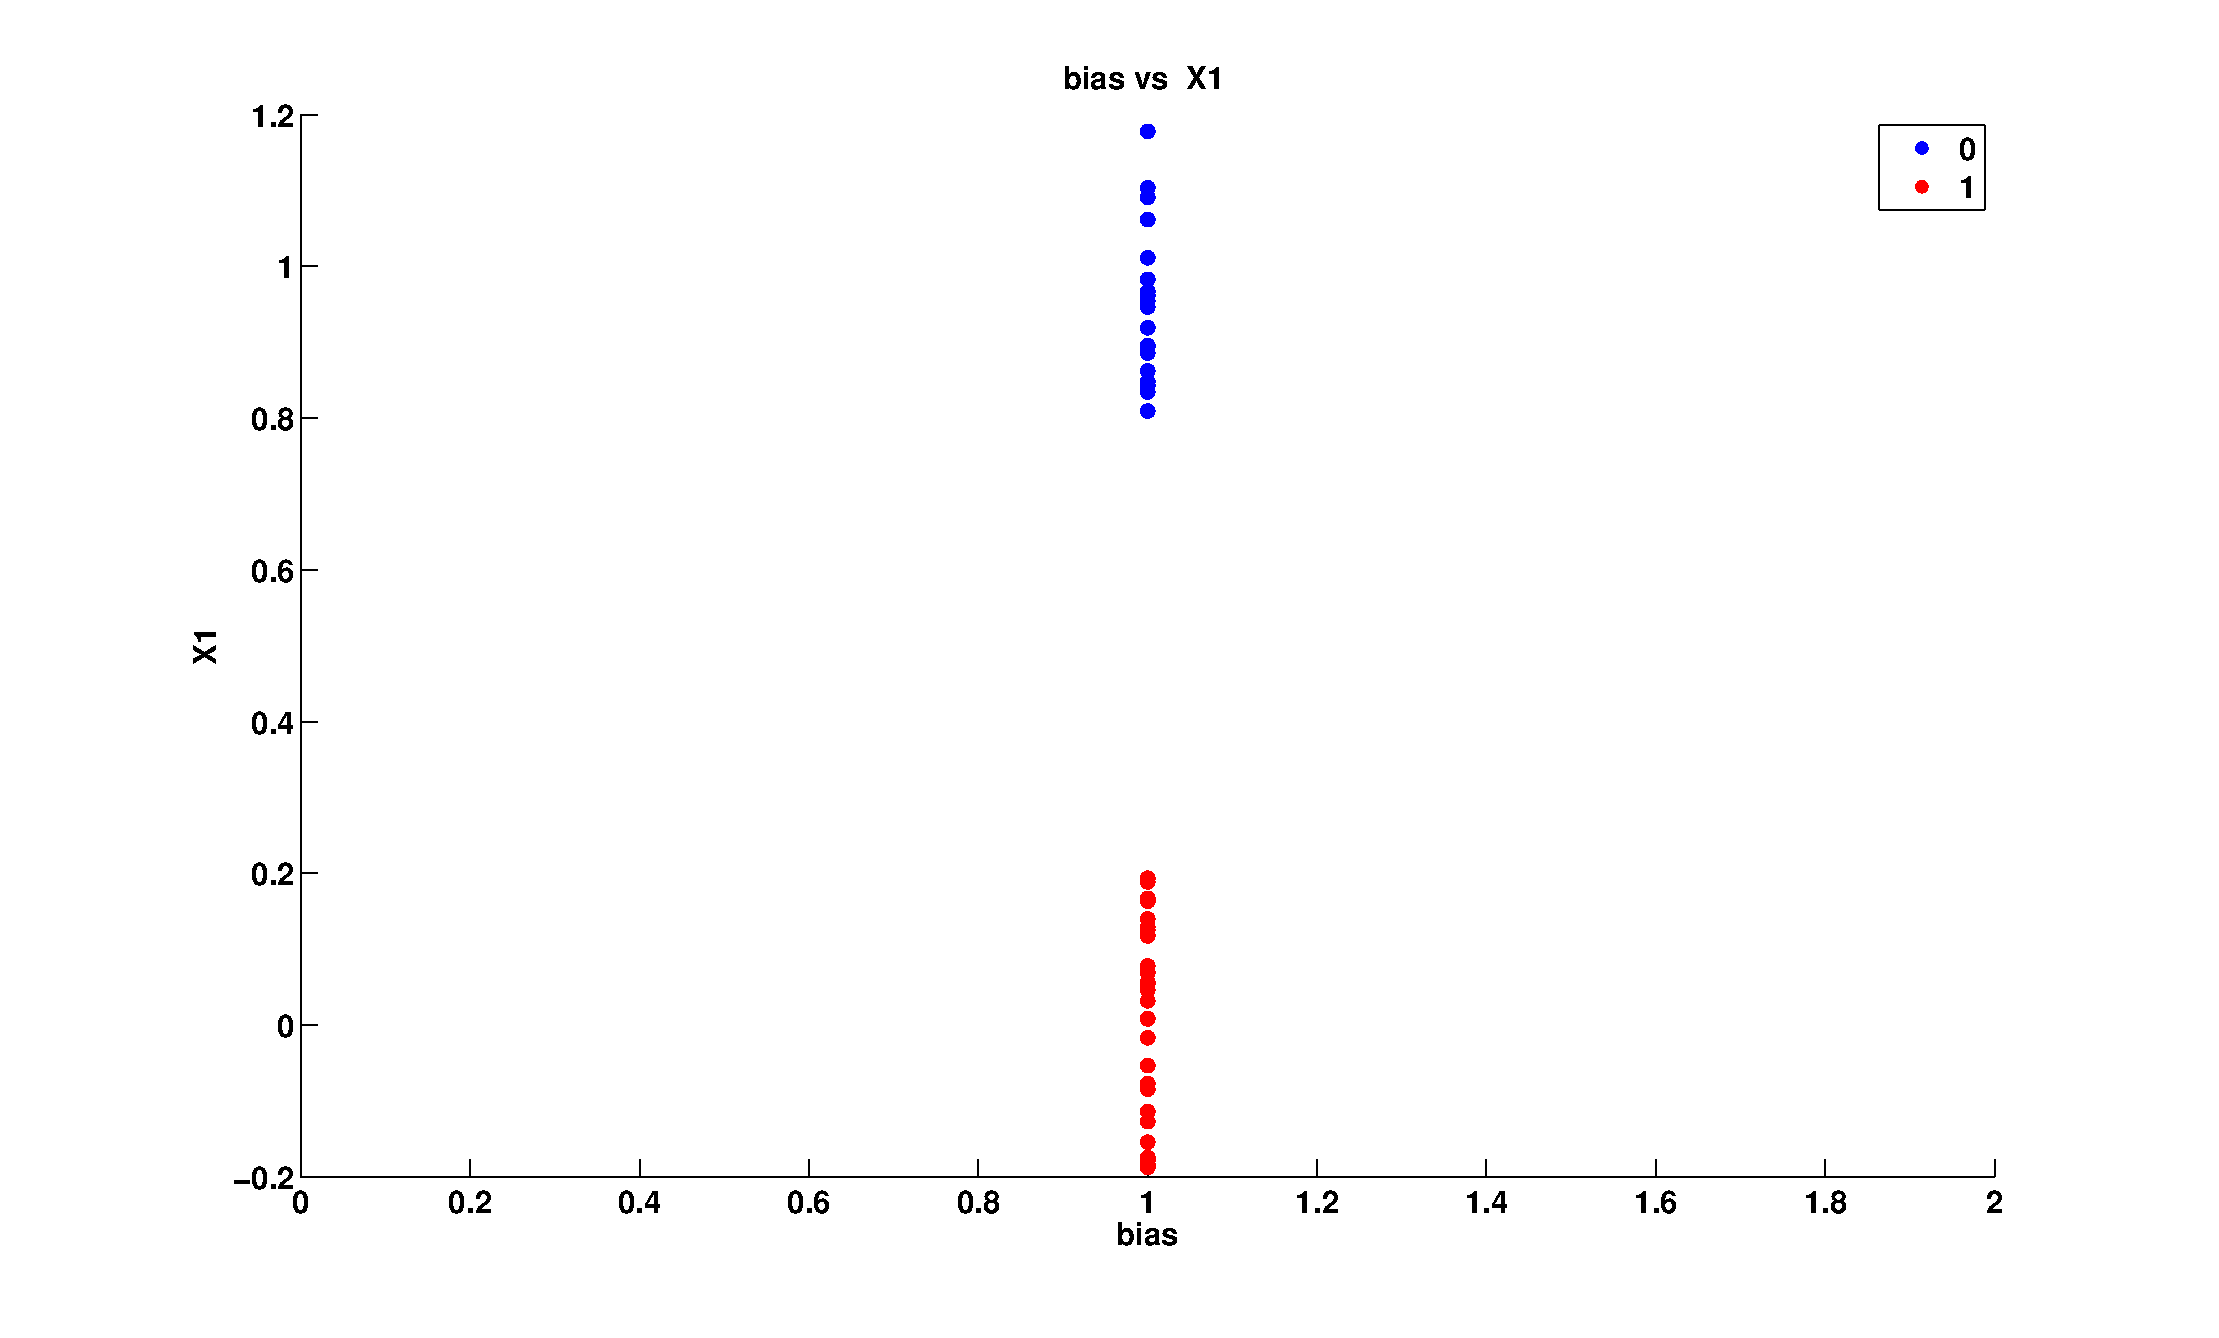
\includegraphics[width=10cm, trim = 3cm 1cm 3cm 1cm, clip=true
	]{eps/not/NOTDesired.eps}
	\caption{Dados utilizados no treinamento. Em vermelho os valores onde o
	operador NOT tem como resultado o valor 1 em função do valor X}
	\label{fig:NOT_dados}
\end{figure} 

A seguir, figura \ref{fig:Not_err} é exibido o erro quadrático médio obtido
durante o treinamento.
É exibido também o erro global, percentual de acerto da época durante o
treinamento usando as amostras de treinamento.
\begin{figure}[!htbp]
	\centering
	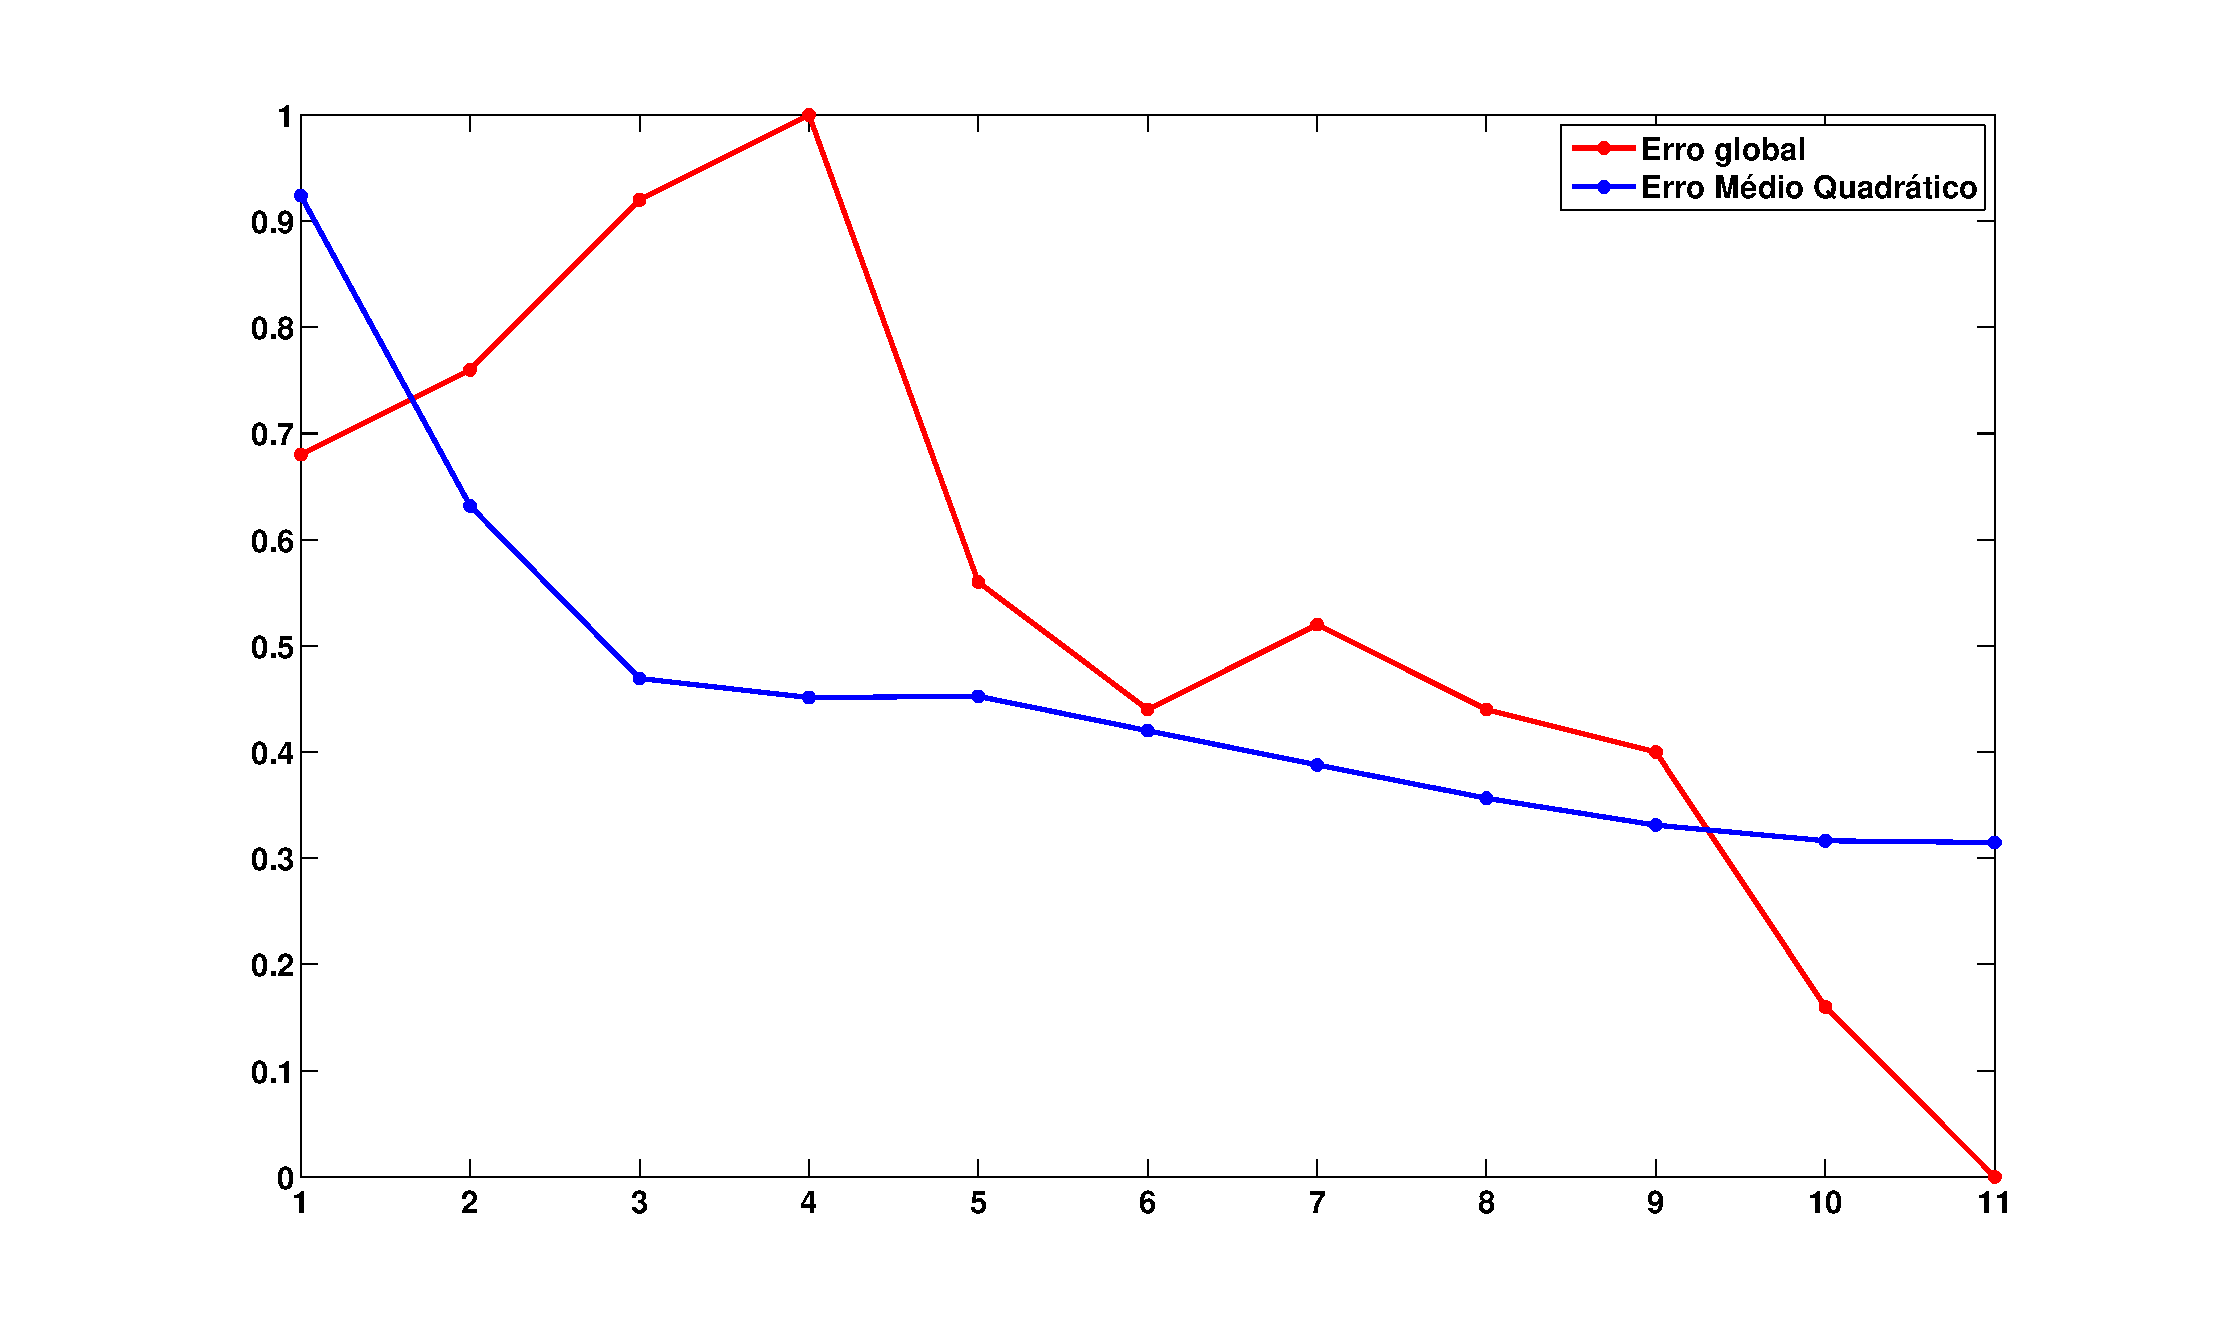
\includegraphics[width=10cm, trim = 3cm 1cm 3cm 1cm, clip=true
	]{eps/not/notErr.eps}
	\caption{Erro obtido durante cada época do treinamento}
	\label{fig:Not_err}
\end{figure} 

Após o treinamento é possível calcular a região de decisão traçada pelo
perceptron, figura \ref{fig:NotReg}.

\begin{figure}[!htbp]
	\centering
	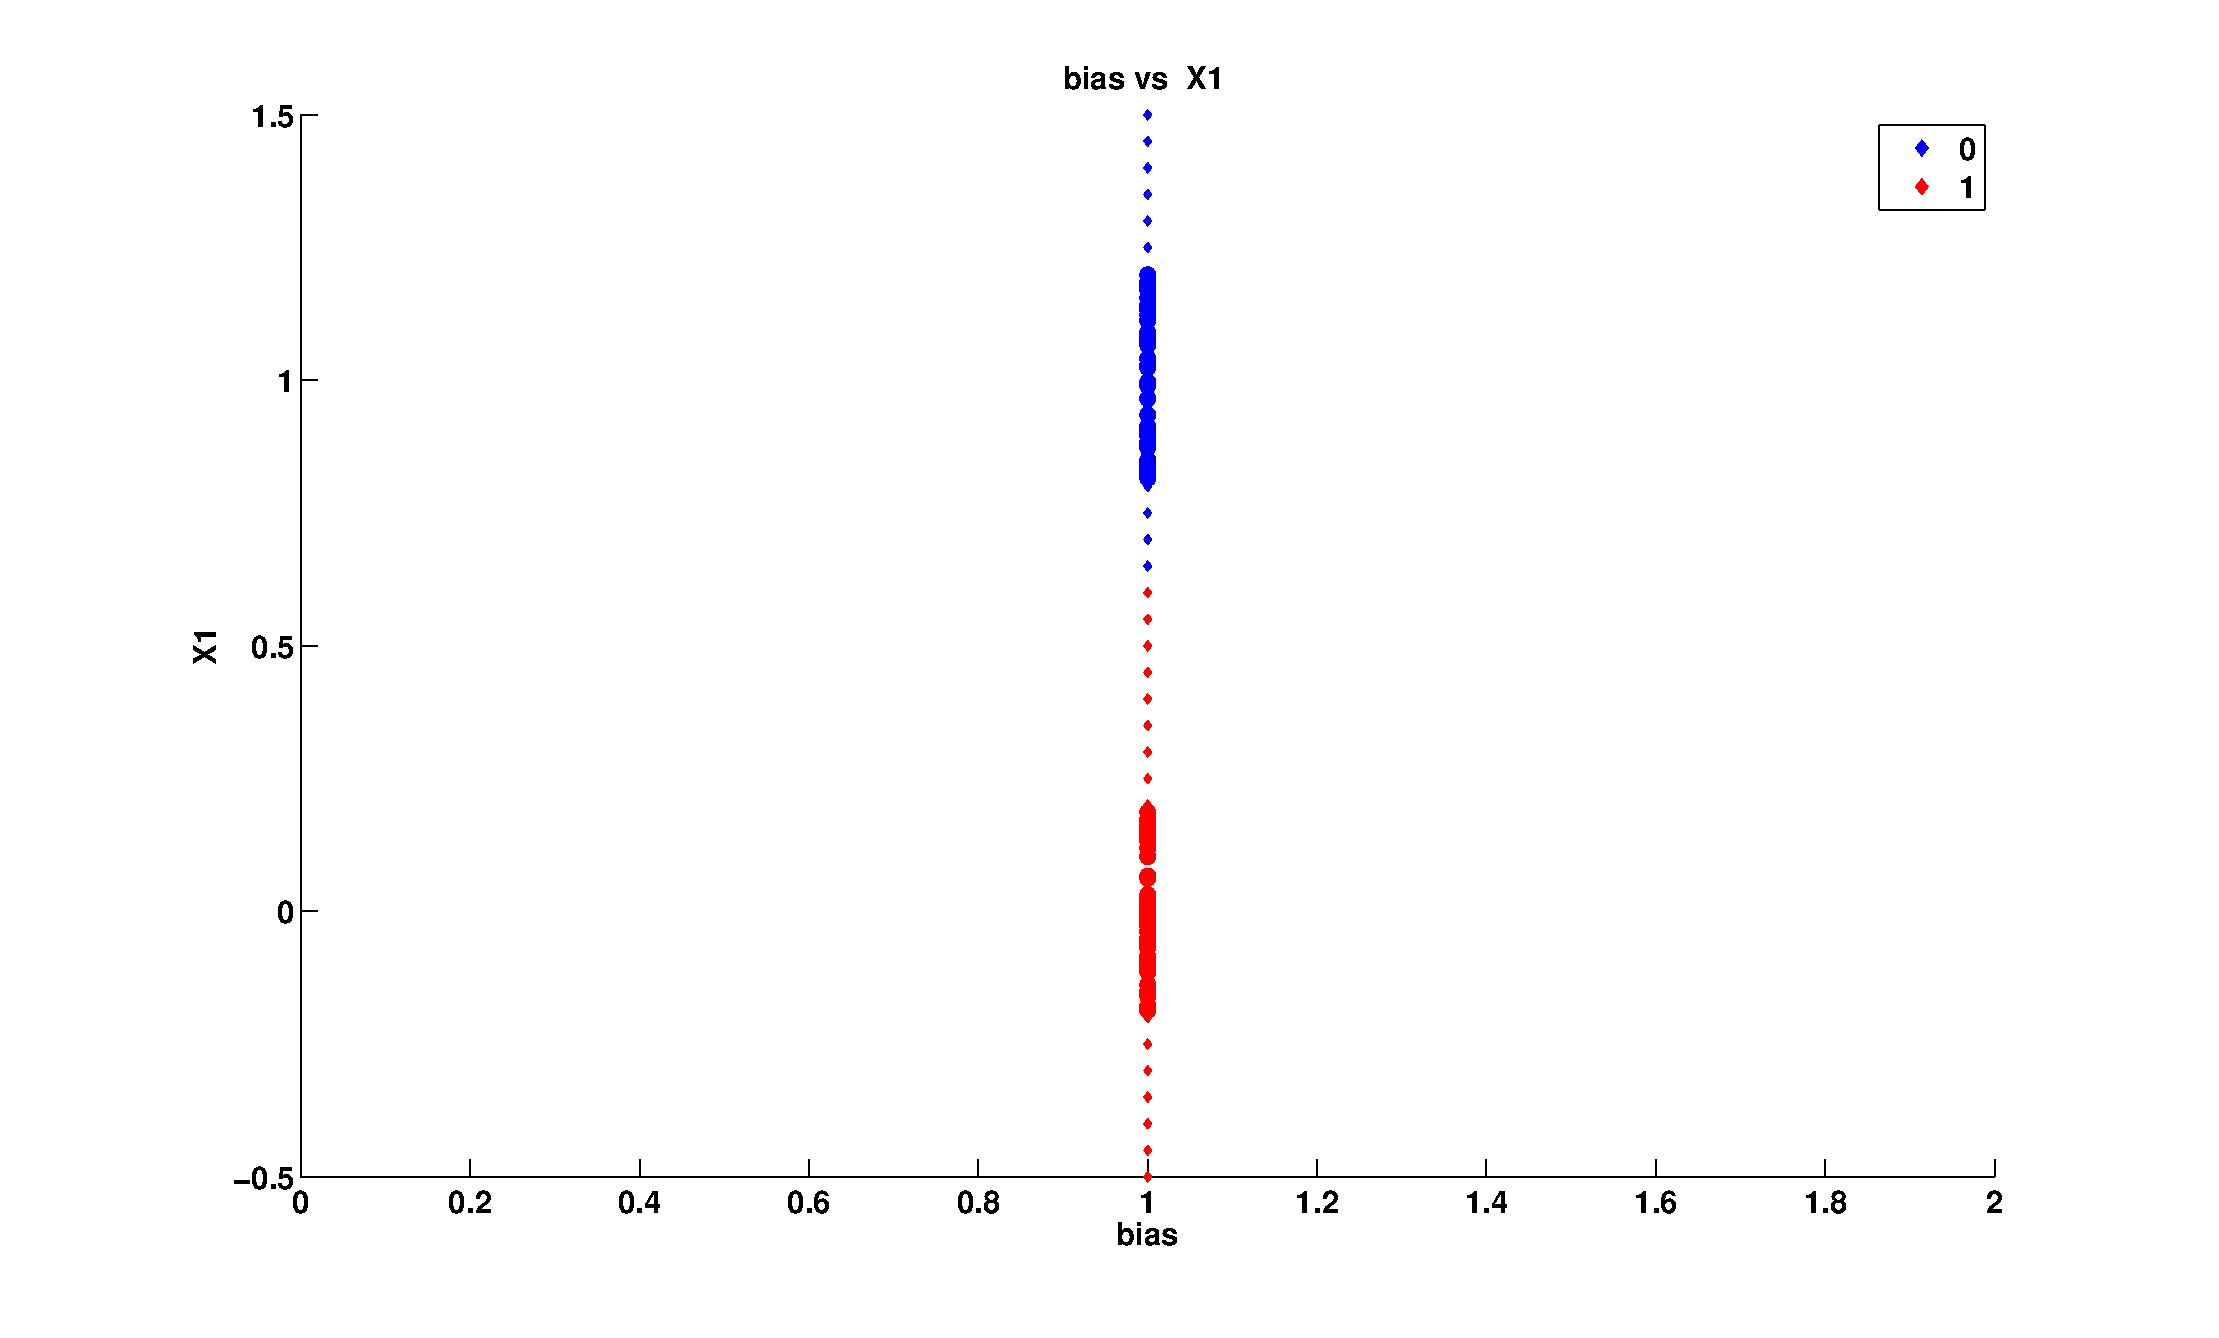
\includegraphics[width=10cm, trim = 3cm 1cm 3cm 1cm, clip=true]
	{eps/not/NOTRegiao.eps}
	\caption{Região de decisão calculada para a porta NOT após o treinamento. O
	fundo pontilhado indica a região de decisão. Em vermelho a região em que as
	amostras são classificadas como 1. Os pontos de raio maior são os dados de
	treinamento.}
	\label{fig:NotReg}
\end{figure} 

Diferentemente dos outros operadores, o operador NOT possui apenas um operando.
Isso faz com que a região de decisão seja apenas uma linha. Na \ref{fig:NotReg}
pode-se perceber que para entradas acima de 0.8 os valores são mapeados  para 0
ao contrário dos valores menores que 0.8 que são mapeados para 1.

\subsection{Setosa vs Outras}
\label{subsec:setOutras}
Este problema consiste em classificar a espécie de Íris Setosa das outras( Íris
Virgínica e Íris Versicolor). O dataset utilizado para o treinamento consiste de
50 amostras de cada uma das três espécies e a classificação será feita com base
nas 4 características disponíveis. Largura e comprimento da pétala e sépala.

Abaixo, na figura \ref{fig:irisDataset} temos a disposição dos dados tendo como
característica as larguras da sépala e pétala. A distribuição de outras
características pode ser visualizada na subsessão \ref{subsec:IrisDataset}
localizada no Apêndice.


\begin{figure}[!htbp]
	\centering
	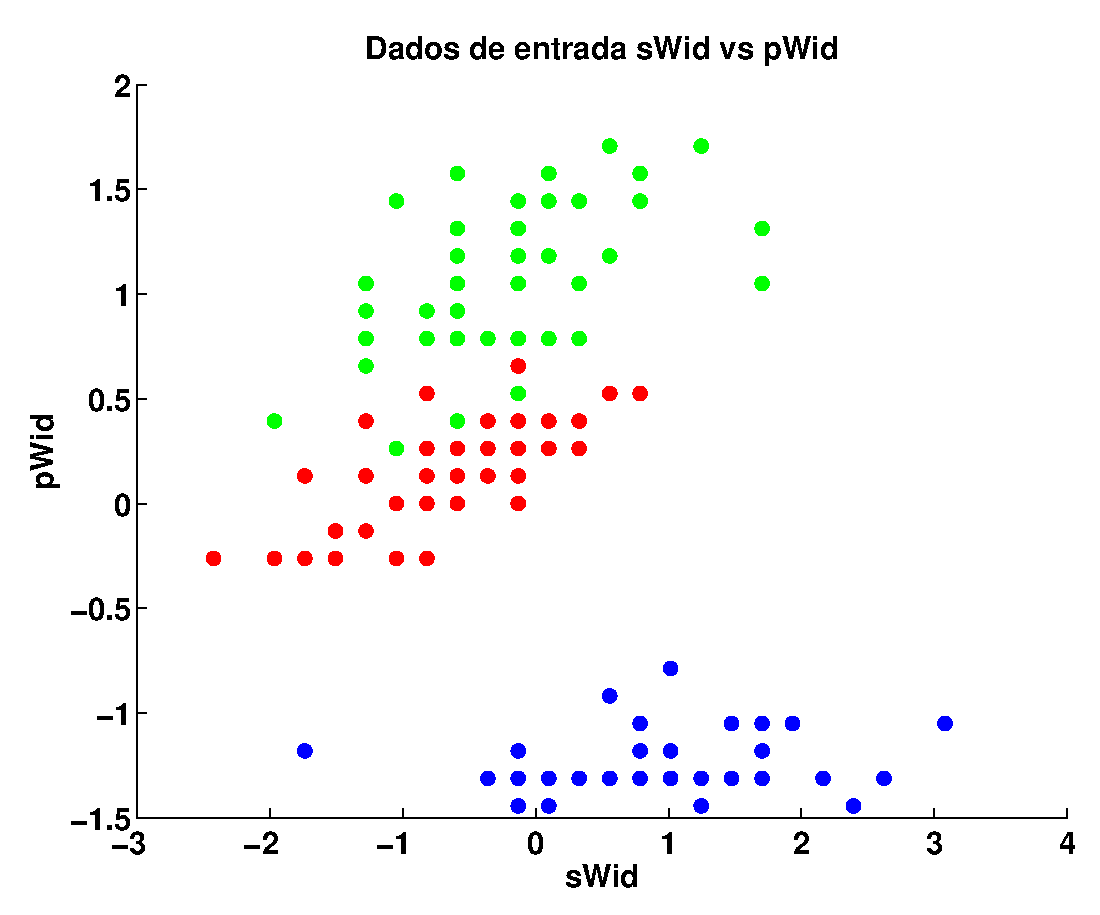
\includegraphics[width=10cm]
	{eps/3classes/input/sWid-vs-pWid.eps}
	\caption{Largura da pétala e sépala da íris. Cada espécie é
	representada por uma cor. Em azul temos a Íris Setosa, em vermelho
	Íris Versicolor e verde a Íris Virgínica.}
	\label{fig:irisDataset} 
\end{figure}

Foi necessário realizar alguns ajustes nos dado de entrada para que ele possa
ser processado pelo perceptron. Para este problema a classe setosa recebeu o
valor 1 como identificador e as outras duas classes receberam o valor 0. Veja a
subsessão \ref{subsec:carregaDataset} localizada no Apêndice.

Os dados coletados foram separados em duas categorias: dados de
treinamento, utilizados para o treinamento do perceptron e dados de teste,
utilizados para verificar sua performance.

Após o treinamento é possível calcular a região de decisão traçada pelo
perceptron, figura \ref{fig:decSetosa}. Os pontos existentes nesta região são os
pontos utilizados como teste. 
 
\begin{figure}[!htbp]
	\centering
	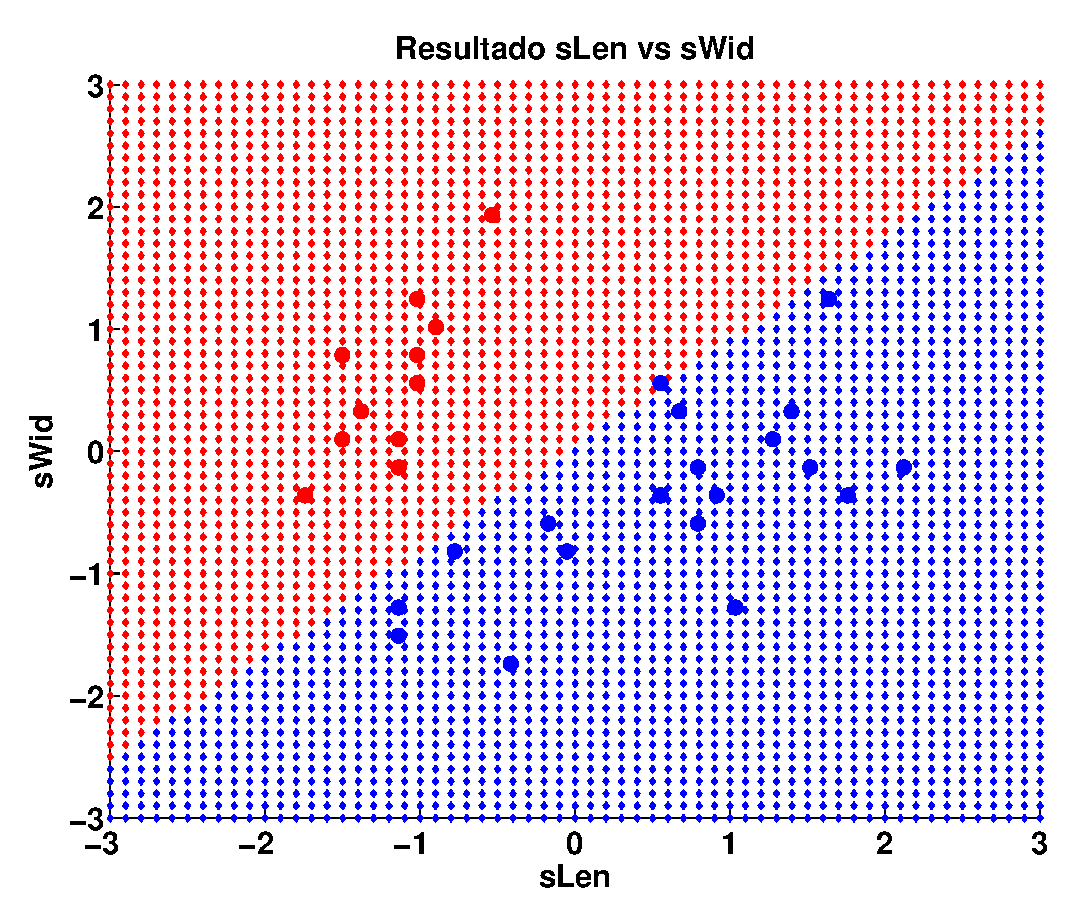
\includegraphics[width=10cm]
	{eps/setosa/regiao/sLen-vs-sWid.eps}
	\caption{Região de decisão calculada para a classe setosa. No eixo vertical
	temos o comprimento da sépala e no eixo horizontal a largura da sépala.}
	\label{fig:decSetosa}
\end{figure} 

A acurácia média e o desvio padrão obtido para 100, 50 e 25 repetições são
exibidas na tabela \ref{tab:acurrSet}  e \ref{tab:acurrSet2} Percebe-se que com
apenas 50\% dos dados para treinamento é possível obter-se uma grande taxa de
acerto, cerca de 98\%.


\begin{table}[!htbp]  
\caption{Resultado da acurácia utilizando 20\%
				 dos dados para treinamento}
\label{tab:acurrSet}
\centering
	\begin{tabular}{| c | c | c |}
		\hline
		 Repetições & Média & Desvio \\ \hline
		 25      & 0.9938   & 0.0128 \\ \hline
		 50      & 0.99     & 0.0194 \\ \hline
		 100 	 & 0.9909   & 0.0179 \\ 
		\hline
	\end{tabular}
\end{table}


\begin{table}[!htbp]  
\caption{Resultado da acurácia utilizando 50\%
				 dos dados para treinamento}						 
\label{tab:acurrSet2}
\centering
	\begin{tabular}{| c | c | c |}
		\hline
		 Repetições & Média & Desvio \\ \hline
		 25      & 0.9875   & 0.0161 \\ \hline
		 50      & 0.9875   & 0.0160 \\ \hline
		 100 	 & 0.9864   & 0.0182 \\ 
		\hline
	\end{tabular}
\end{table}


\subsection{Adaline}
O Adaline difencia-se do perceptron basicamente pelo não uso da função de
ativação. Durante a fase de aprendizagem o adaline ajusta o pesos de acordo com
o erro e o valor da entrada. O Adaline assim como o perceptron aceita várias
entradas e apenas uma saída. Se a diferença entre a saída desejada e o valor
calculado for maior que um dado limiar os pesos das entradas são atualizados.
O Adaline tem como principal utilização a aproximação de funções lineares.
Na figura \ref{fig:regressao} é exibido um comportamento aproximado da seguinte
função $f(x)=3 \times x + 8$. Os dados exibidos na figura foram utilizados no
treinamento, o qual gerou o gráfico plotado na figura \ref{fig:regressaoErro}.
Na figura \ref{fig:regressaoResultado} é exibido o resultado após o treinamento
do Adaline. Vale ressaltar que após o treinamento os valores dos pesos do
Adaline são os coeficientes da função linear aproximada por ela.

\begin{figure}[!htbp]
	\centering
	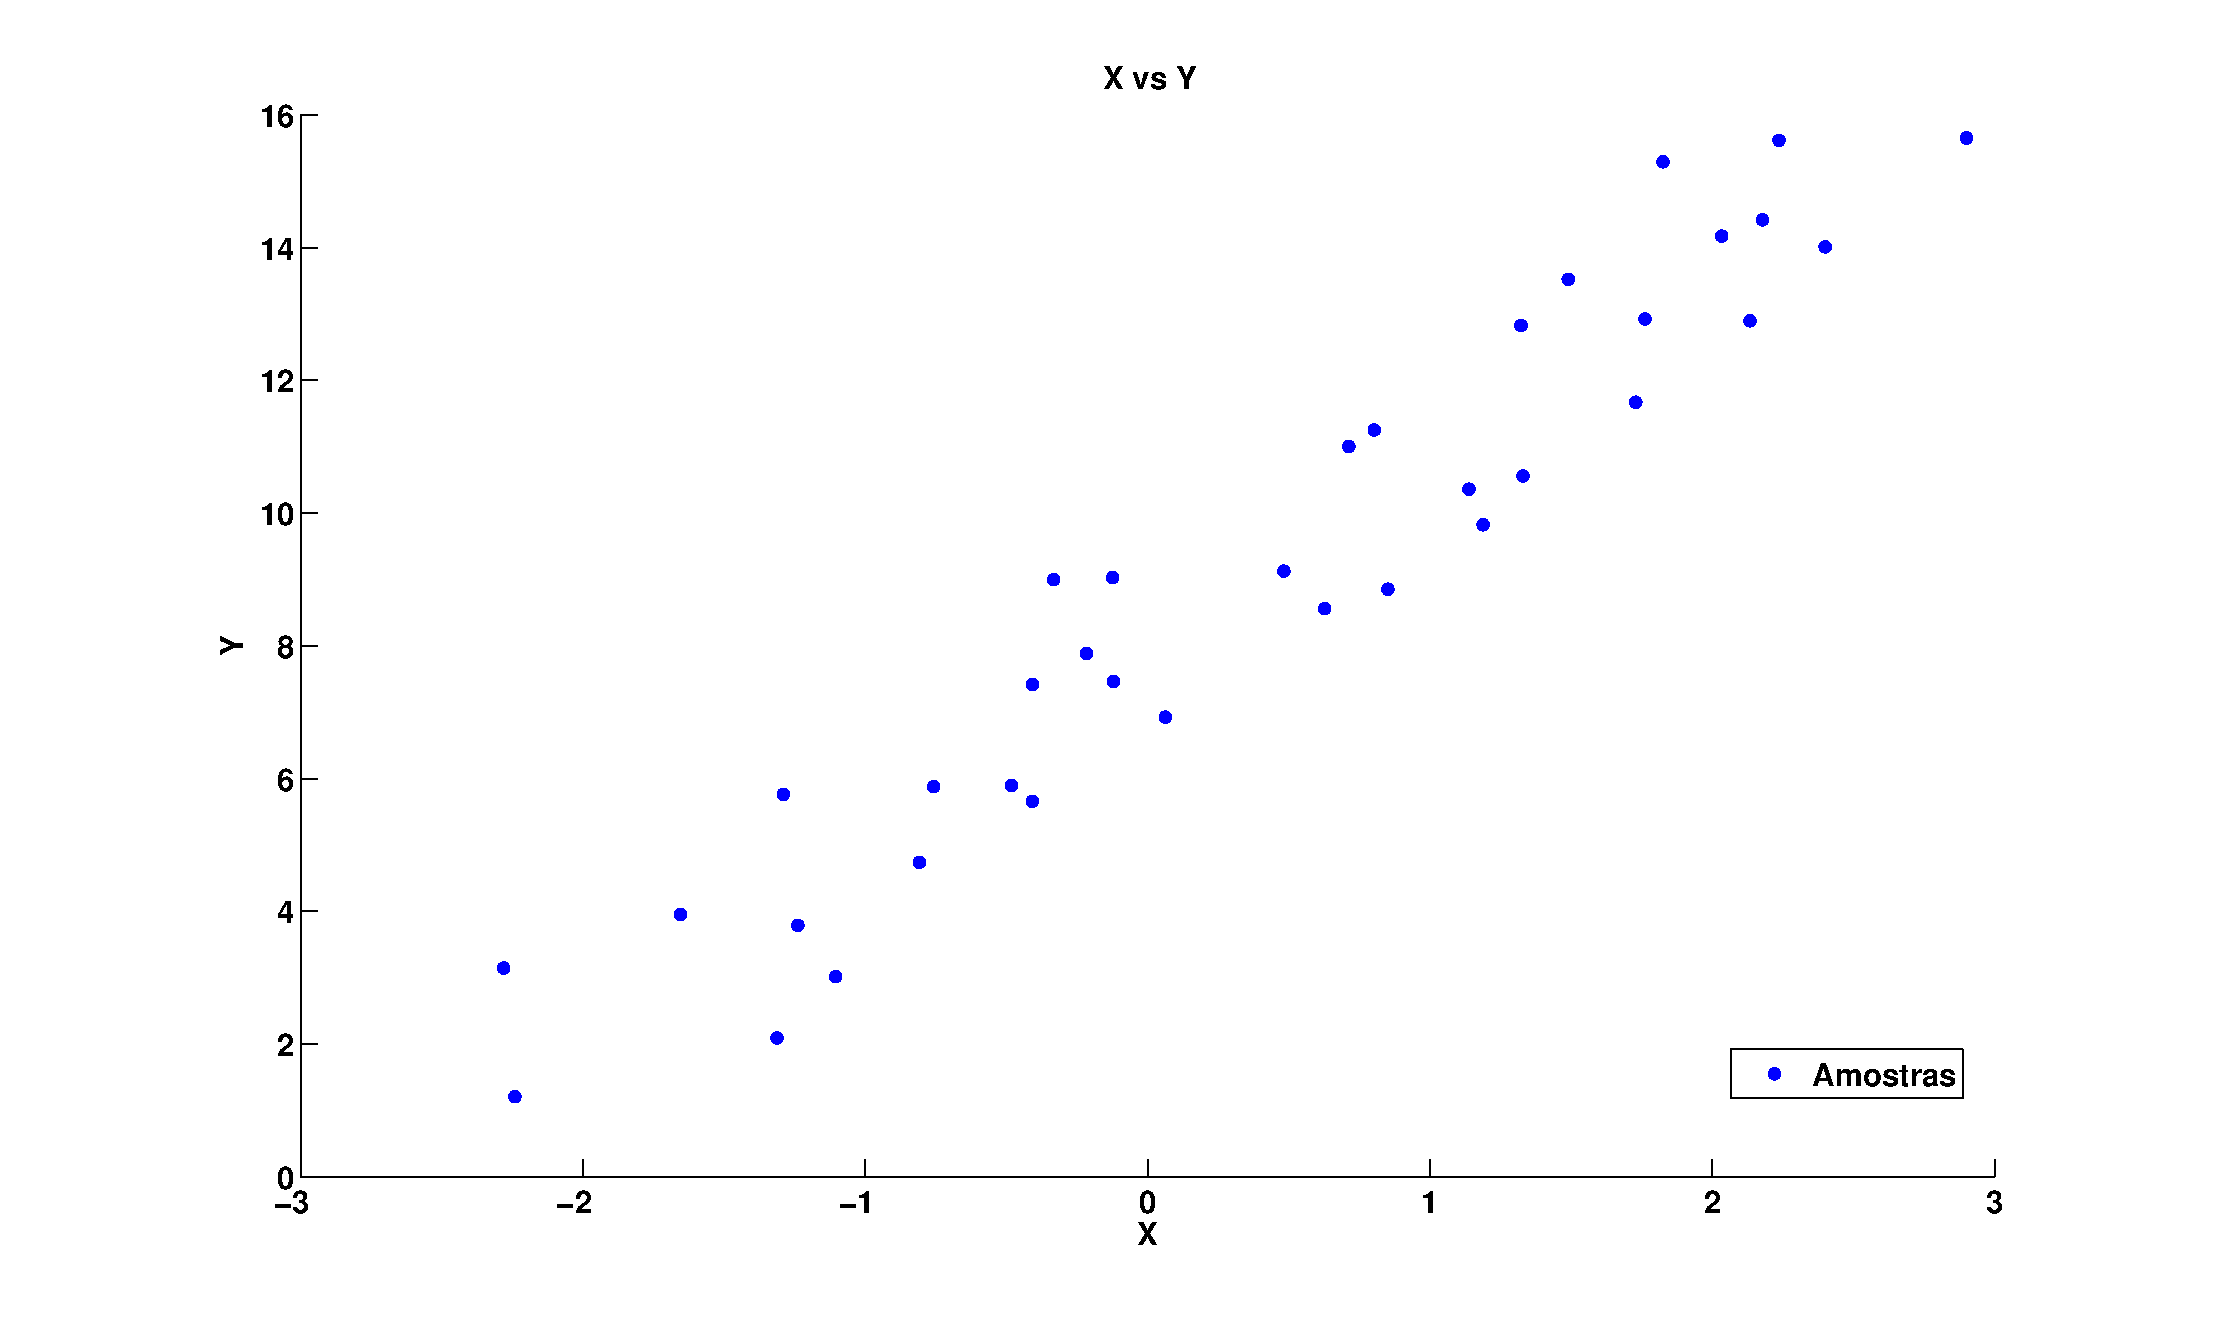
\includegraphics[width=10cm, trim = 3cm 1cm 3cm 1cm, clip=true]
	{eps/adaline/amostras.eps}
	\caption{Dados utilizados para o treinamento do Adaline.}
	\label{fig:regressao} 
\end{figure}

\begin{figure}[!htbp]
	\centering
	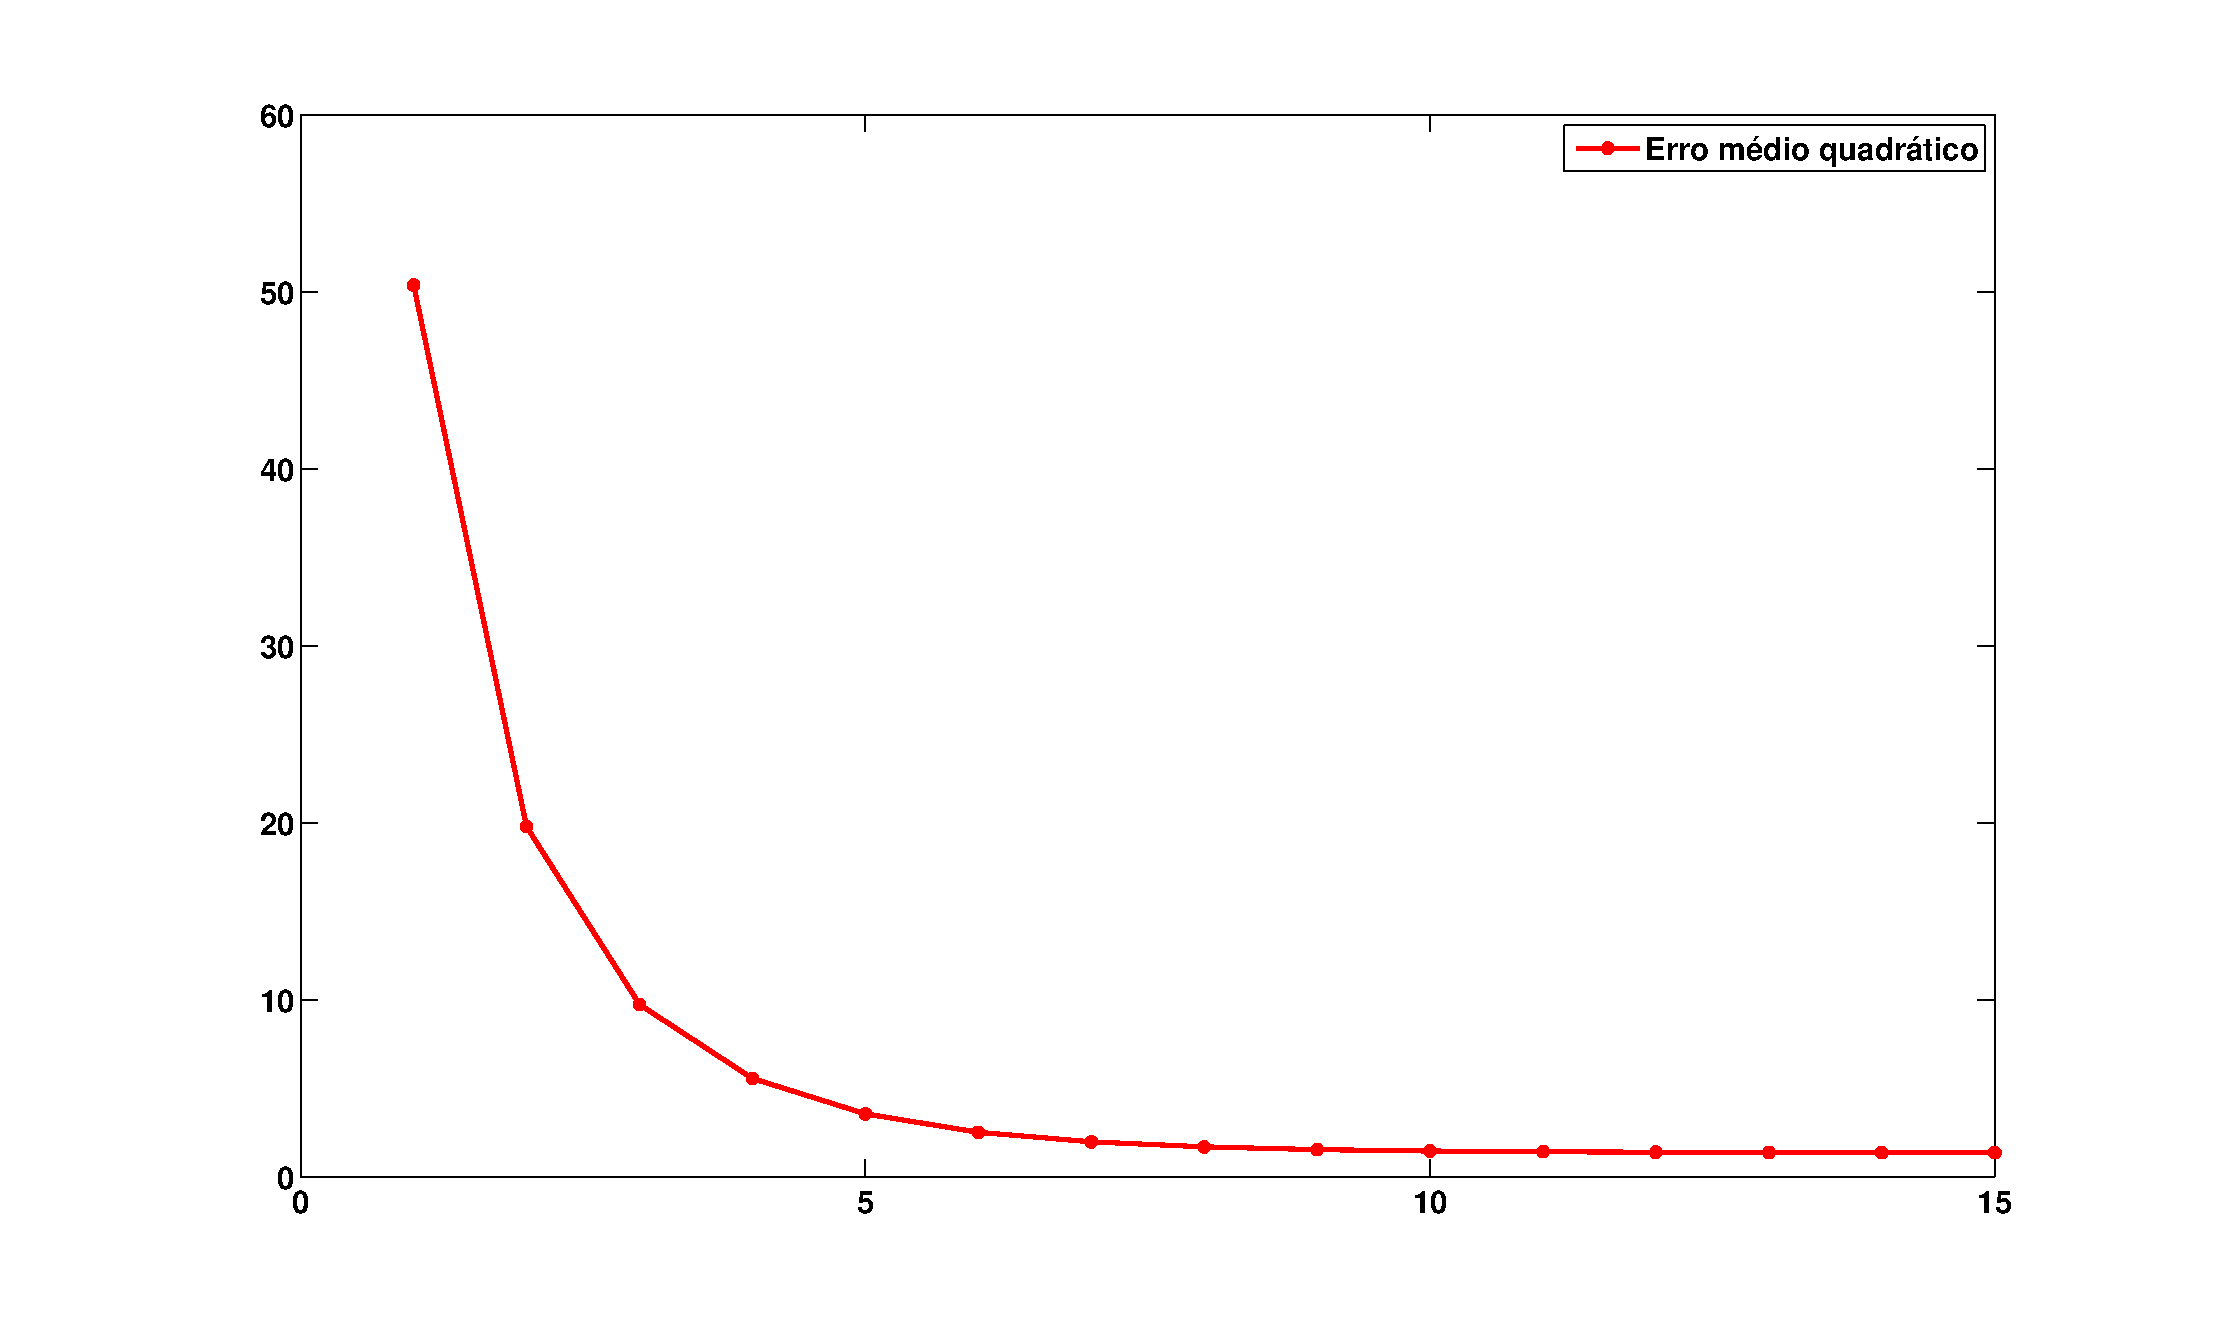
\includegraphics[width=10cm, trim = 3cm 1cm 3cm 1cm, clip=true]
	{eps/adaline/erro.eps}
	\caption{Erro médio quadrático gerado durante o treinamento do Adaline.}
	\label{fig:regressaoErro} 
\end{figure} 

\begin{figure}[!htbp]
	\centering
	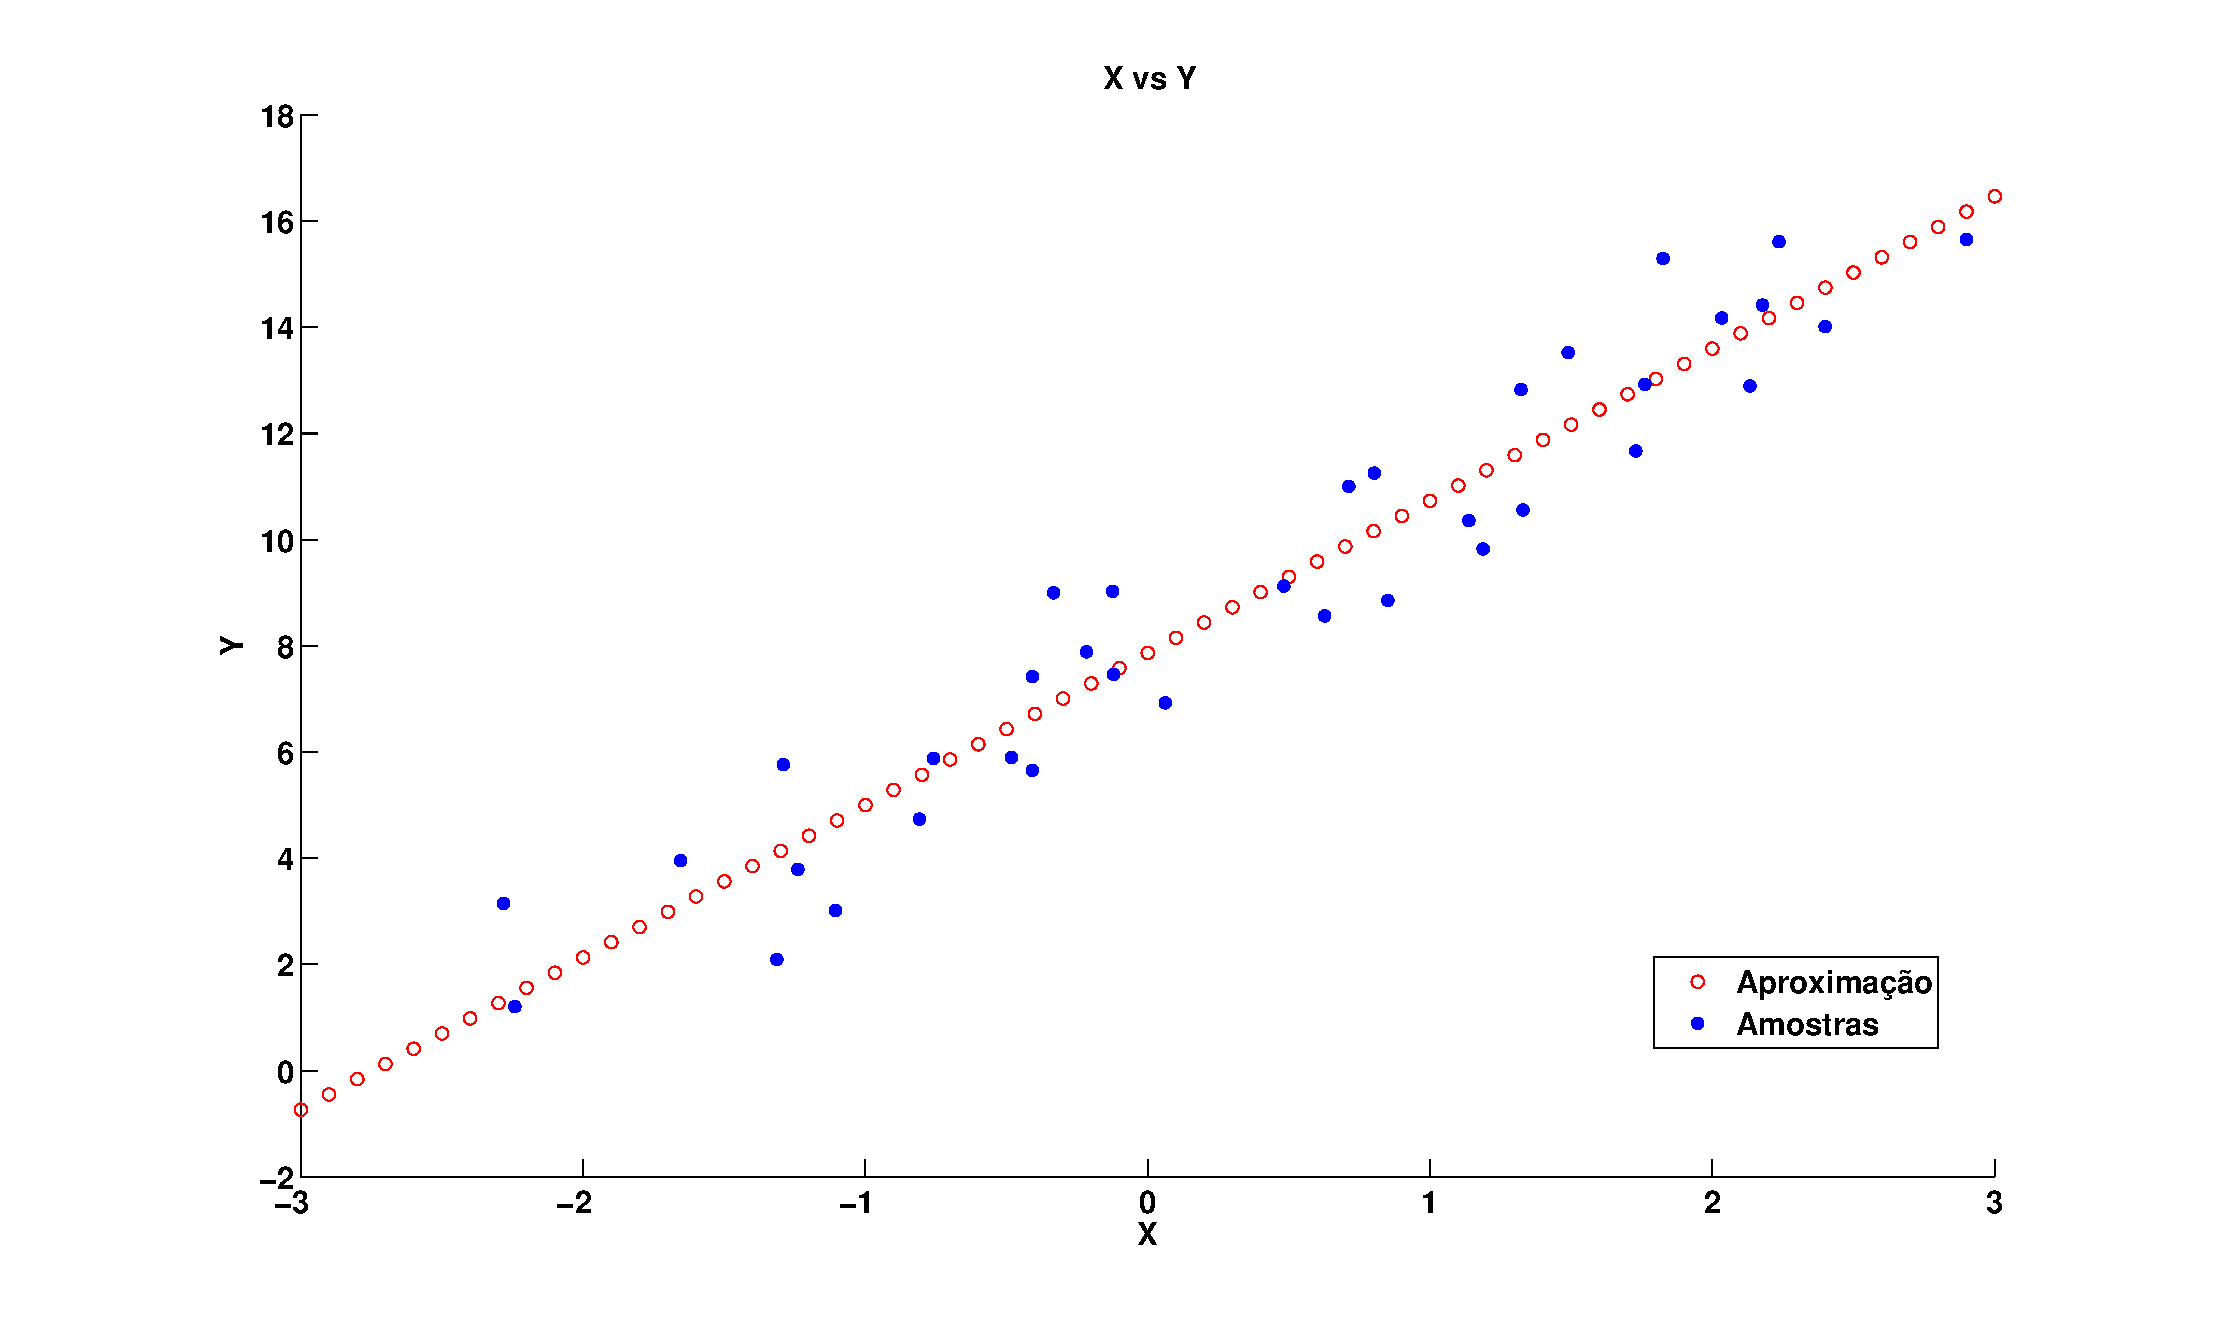
\includegraphics[width=10cm, trim = 3cm 1cm 3cm 1cm, clip=true]
	{eps/adaline/resultado.eps}
	\caption{Resultado após o treinamento. Em vermelho temos a reta aproximada aos
	dados.}
	\label{fig:regressaoResultado} 
\end{figure} 


\subsection{Setosa vs Virgínica vs Versicolor}
Este problema consiste em classificar as espécie de Íris individualmente,
Íris Setosa Íris Virgínica e Íris Versicolor. O conjunto de dados utilizados é o
mesmo utilizado na subsessão \ref{subsec:setOutras}.

Na figura \ref{fig:irisDataset} temos a disposição dos dados tendo como
característica as larguras da sépala e pétala. A distribuição de outras
características pode ser visualizada na subsessão \ref{subsec:IrisDataset}
localizada no Apêndice.

Os ajustes necessários para o treinamento foram feitos no momento que o dataset
é carregado pela aplicação. Desta vez foram utilizados 3 perceptrons fazendo
com que a saída desejada seja mapeada da forma exposta na tabela \ref{tab:mapMLP}.
Veja o Apêndice \ref{subsec:carregaDataset} para mais detalhes de como é feito o tratamento do dataset.

Para a solução deste problema serão utilizados 3 perceptrons dispostos de acordo
com a figura \ref{fig:mlp}.

\begin{table}[!htbp]  
\caption{Mapeamento da saída de acordo com a classe da Íris.}						 
\label{tab:mapMLP}
\centering
	\begin{tabular}{| c | c | c | c |}
		\hline
		 Tipo 		 &	$y1$ & 	$y2$ 	& 	$y3$ \\ \hline
		 Setosa      & 	1 	 & 	0		&	0 \\ \hline
		 Versicolor  & 	0 	 & 	1		&	0 \\ \hline
		 Virgínica 	 & 	0 	 & 	0		&	1 \\ 
		\hline
	\end{tabular}
\end{table}



\begin{figure}[!htbp]
	\centering
	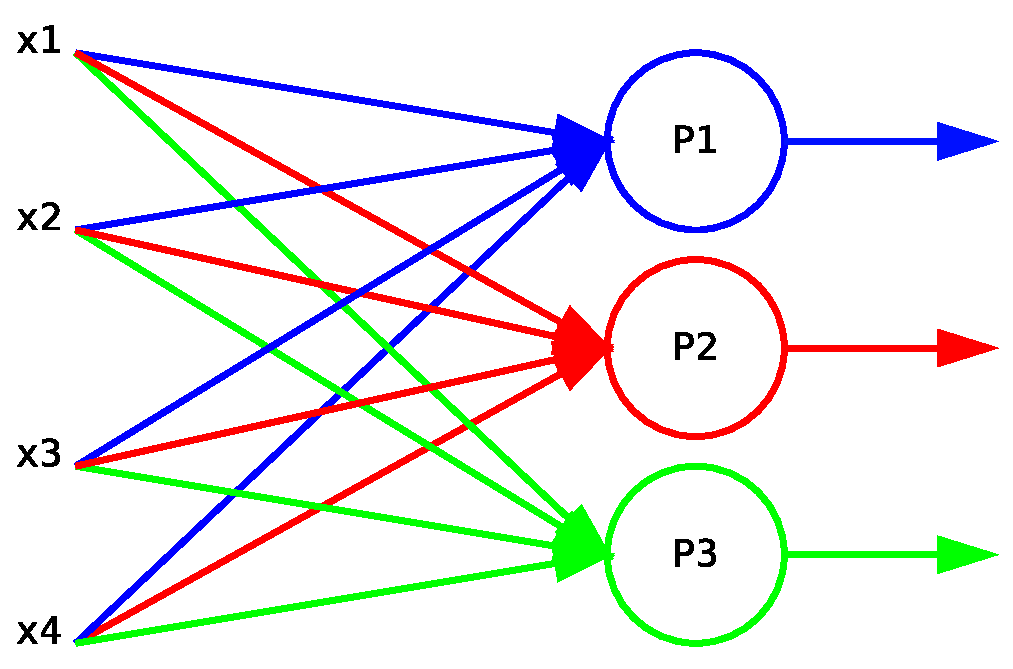
\includegraphics[width=10cm]
	{eps/3classes/mlp.eps}
	\caption{Perceptrons utilizados para realizar a classificação das espécies de
	Íris. O perceptron P1, P2 e P3 classificam a espécie setosa, virgínica
	e versicolor respectivamente.}
	\label{fig:mlp} 
\end{figure} 

Neste modelo pode-se perceber que os perceptrons são independentes entre si.
Cada um, assim como o problema relatado na subssessão \ref{subsec:setOutras}, é
responsável por verificar se aquele dado de entrada pertence a classe na qual o
perceptron foi treinado. Após o treinamento obtemos o seguinte gráfico do erro
quadrático médio.


\begin{figure}[!htbp]
	\centering
	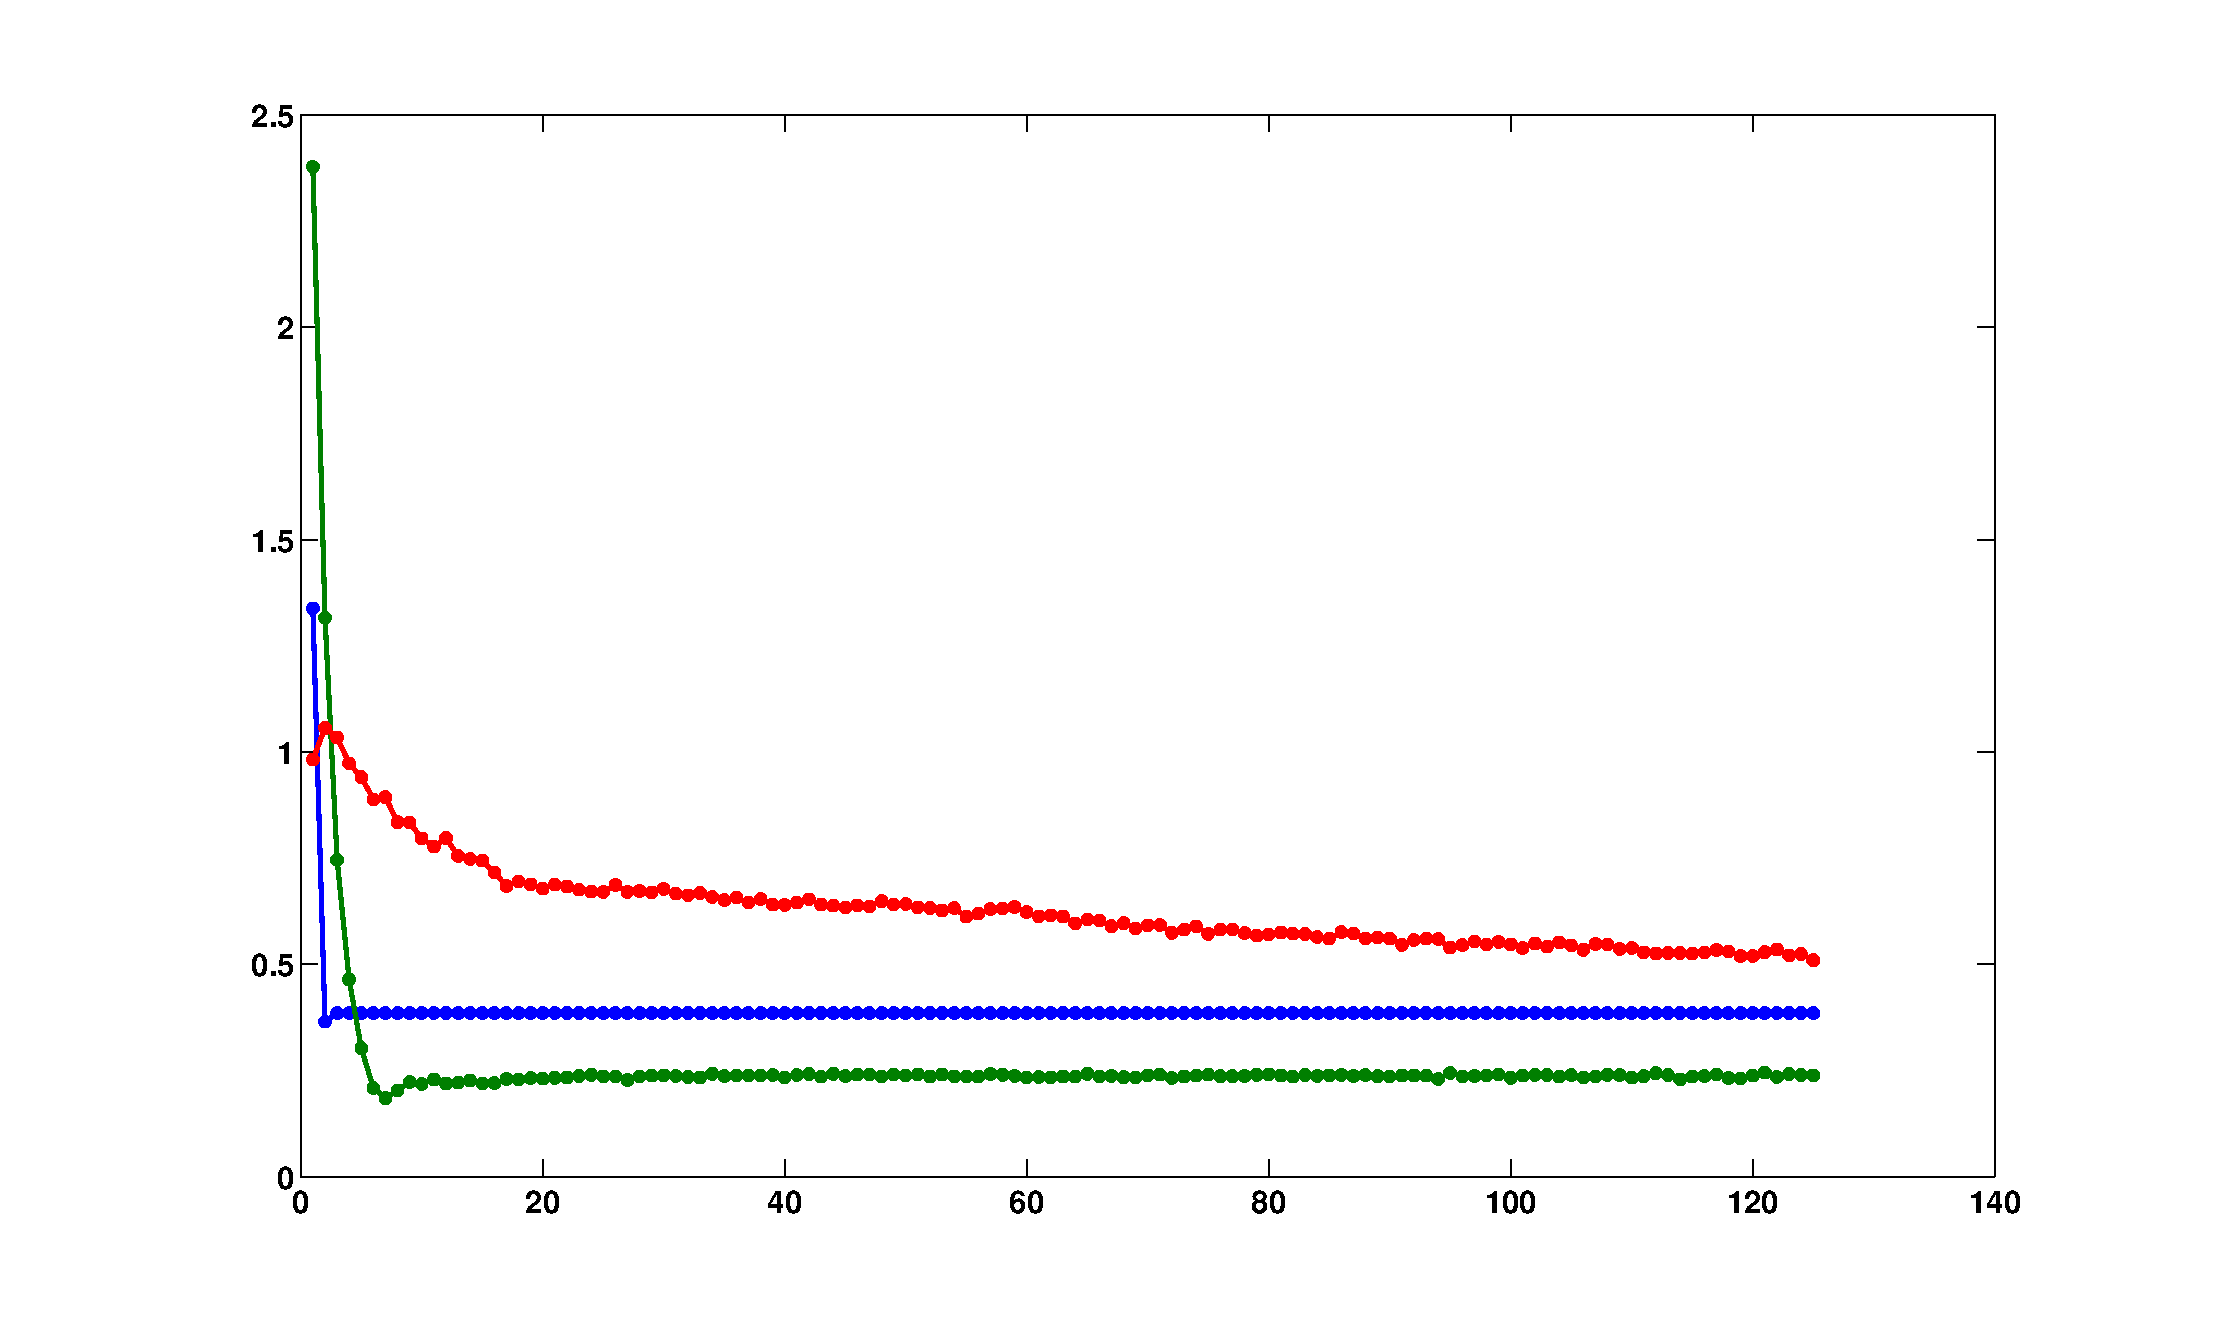
\includegraphics[width=10cm]
	{eps/3classes/erro.eps}
	\caption{Em vermelho o erro médio quadrático obtido durante o treinamento
	para o perceptron da classe Setosa, em azul e verde as classes versicolor e
	vigínica respectivamente.}
	\label{fig:erromlp} 
\end{figure} 



A acurácia média e o desvio padrão obtido para 100,50 e 25 repetições são
exibidas na tabela \ref{tab:acurr3}  e \ref{tab:acurr32} Percebe-se que não foi
possível obter um resultado melhor que 65 \%. Este resultado é esperado tendo em
vista que as classes virgínica e versicolor não podem ser separadas linearmente.


\begin{table}[!htbp]  
\caption{Resultado da acurácia utilizando 20\%
				 dos dados para treinamento das 3 classes de Íris}
\label{tab:acurr3}
\centering
	\begin{tabular}{| c | c | c |}
		\hline
		 Repetições & Média & Desvio \\ \hline
		 25      & 0.6212   & 0.0767 \\ \hline
		 50      & 0.6331   & 0.0808 \\ \hline
		 100 	 & 0.6431   & 0.0795 \\ 
		\hline
	\end{tabular}
\end{table}


\begin{table}[!htbp]  
\caption{Resultado da acurácia utilizando 50\%
				 dos dados para treinamento das 3 classes de Íris}						 
\label{tab:acurr32}
\centering
	\begin{tabular}{| c | c | c |}
		\hline
		 Repetições & Média & Desvio \\ \hline
		 25      & 0.6270   & 0.0877 \\ \hline
		 50      & 0.6247   & 0.0778 \\ \hline
		 100 	 & 0.6227   & 0.0807 \\ 
		\hline
	\end{tabular}
\end{table}

\section{Conclusão}
Este trabalho permitiu fazermos uma análise do perceptron e do adaline. Foi
percebido ao longo do trabalho a grande capacidade do perceptron de realizar a
separação linear de duas classes. Por parte do adaline foi dado um exemplo de
como se fazer a aproximação de funções lineares dado uma distribuição de dados.
Foi apresentado também o resultado da classificação de 3 classes sendo 2 delas
não separável linearmente, utilizando 3 perceptrons. Foi verificado um resultado
não satisfatório para esta classificação.
%\section{Resultados}
%\section{Conclusão}
\afterpage
\onecolumn




% you can choose not to have a title for an appendix
% if you want by leaving the argument blank
\section{Apêndice}

\subsection{Gera Base de Treinamento}
\label{subsec:geraBase}
Abaixo é possível visualizar o código implementado em Matlab para gerar a base
de dados para os operadores AND, OR e NOT. 
Através do parâmetro tipo é possível selecionar o tipo de base de dados que será
gerado. As opções são AND, OR e NOT. Para a base NOT é importante ressaltar que
os valores de X apresentam apenas uma dimensão.
A base de dados gera uma nuvem em torno dos valores 0 e 1 com variação de até
0.2, isso é feito nos passos da linha 4 à 7. Após a criação da núvem é feita uma
operação utilizando os operadores do matlab.

\lstinputlisting[]
{code/perceptron/geraBD.m}

\subsection{Carrega Dataset} 
\label{subsec:carregaDataset}
Abaixo é possível visualizar o código implementado em Matlab para carregar os
dados da Íris. De acordo com o valor da variável \textit{modo}, a saída y, utilizada
como saída deseja pelo classificador, é alterada.
\lstinputlisting[]
{code/mlp/carregaDados.m}



\subsection{Características Combinadas para o DataSet da Íris}
\label{subsec:IrisDataset}

Abaixo temos as caractéristicas do DataSet da Íris combinados. É fácil perceber
que a classe que está em azul(Setosa) é linearmente separável em praticamente
qualquer combinação de características. Diferentemente das outras duas classes,
Versicolor e Vigínica que têm uma região em comum em várias características
principalmente quando relacionamos o comprimento com a largura da sépala.

\begin{figure}[h]
	\centering
	\begin{subfigure}[h]{0.3\textwidth}
		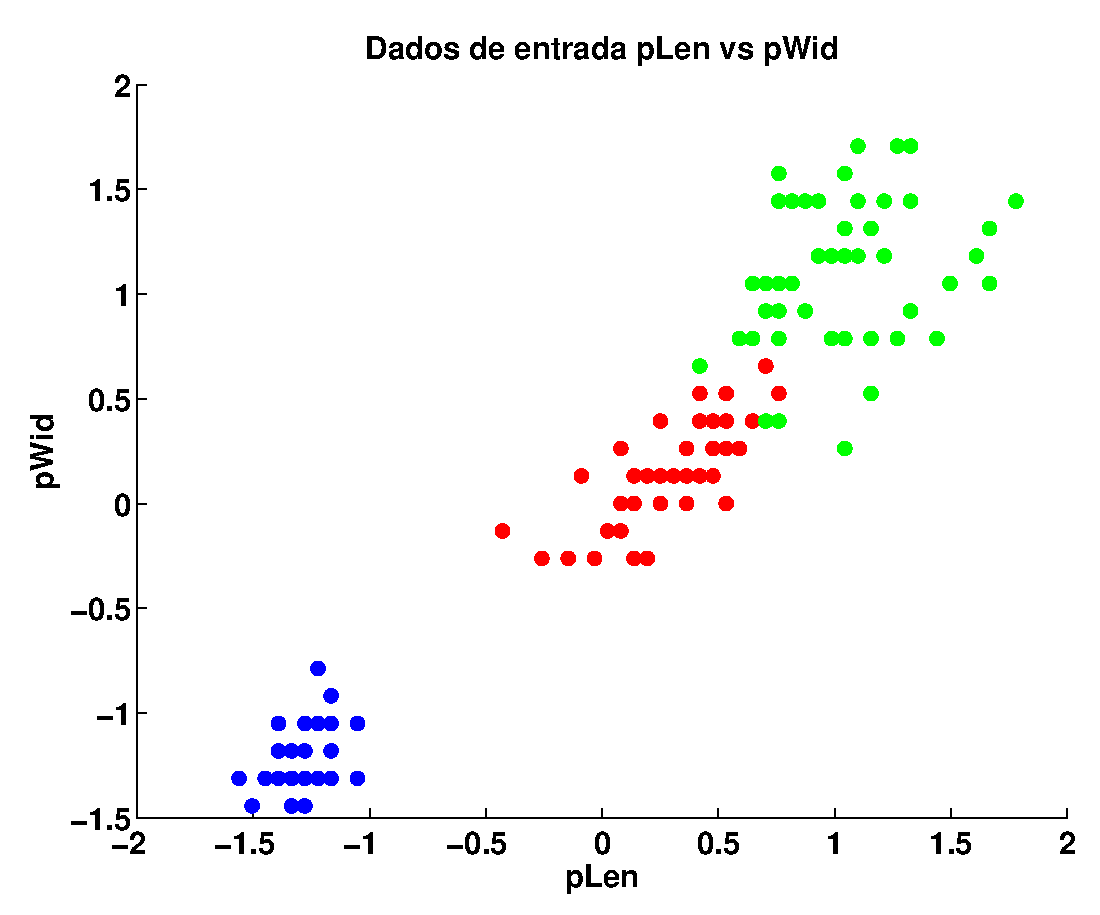
\includegraphics[width=\textwidth]{eps/3classes/input/pLen-vs-pWid.eps}
	\end{subfigure} 
	\begin{subfigure}[h]{0.3\textwidth}
		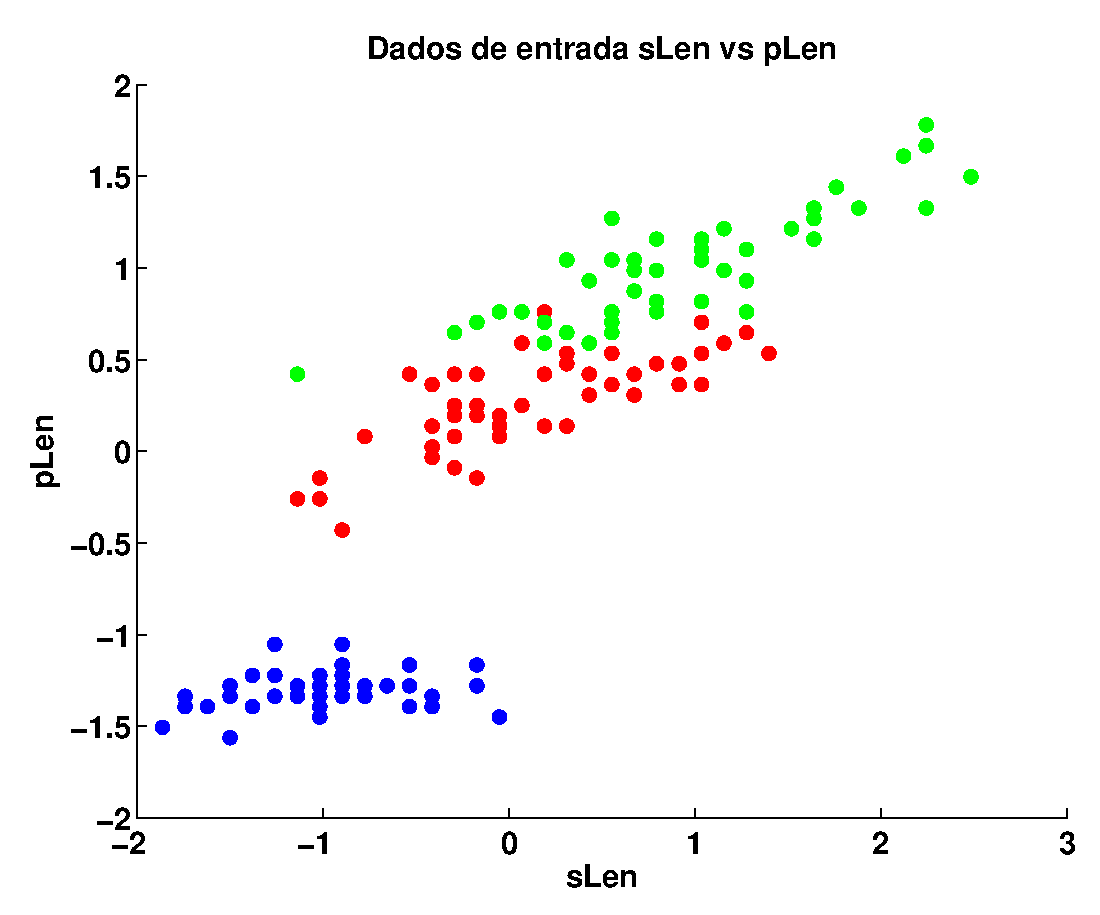
\includegraphics[width=\textwidth]{eps/3classes/input/sLen-vs-pLen.eps}
	\end{subfigure} 
	\begin{subfigure}[h]{0.3\textwidth}
		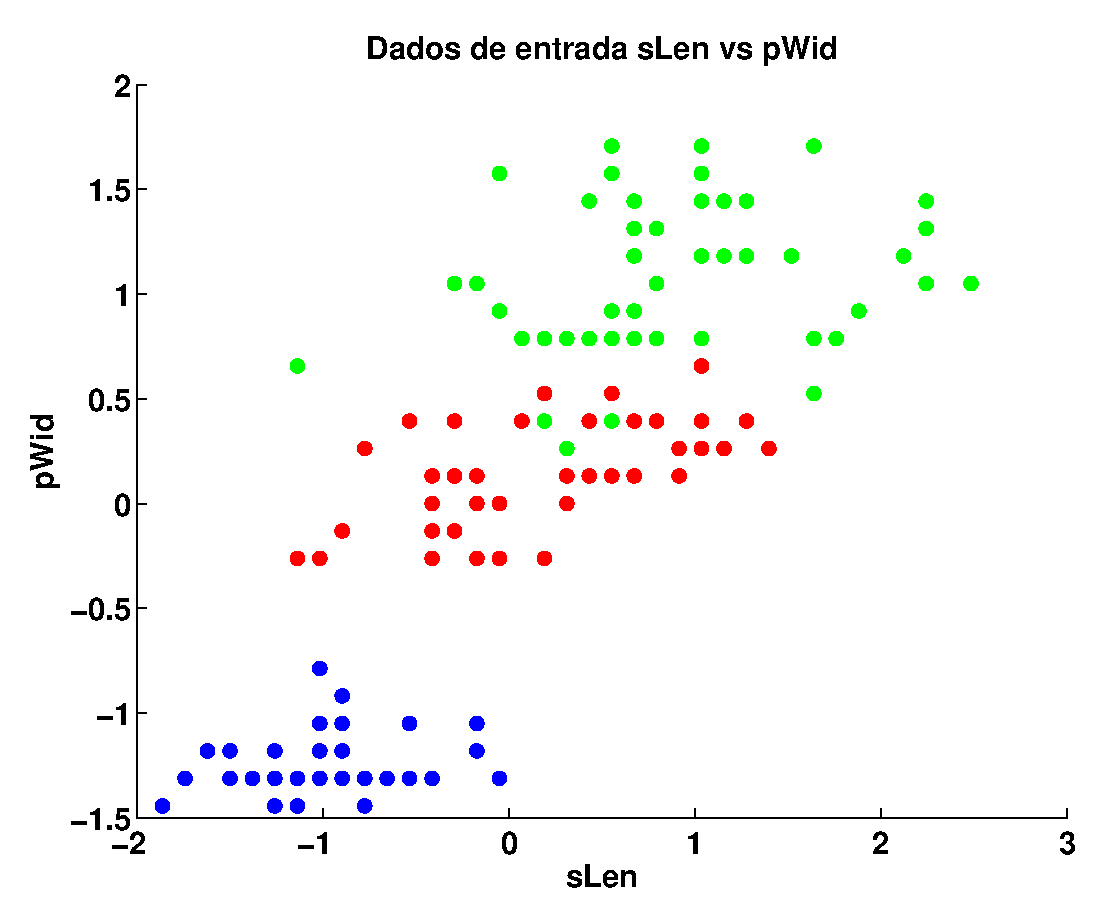
\includegraphics[width=\textwidth]{eps/3classes/input/sLen-vs-pWid.eps}
	\end{subfigure} 
	
	\begin{subfigure}[h]{0.3\textwidth}
		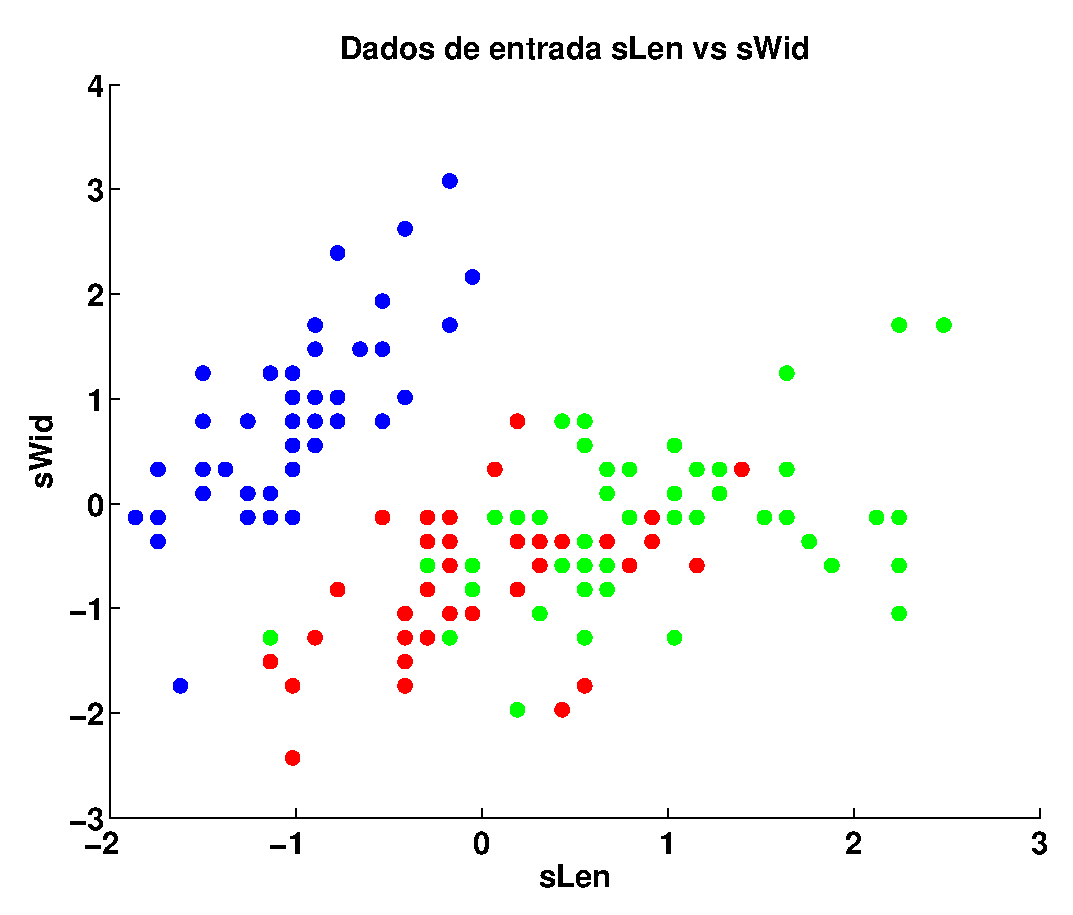
\includegraphics[width=\textwidth]{eps/3classes/input/sLen-vs-sWid.eps}
	\end{subfigure} 
	\begin{subfigure}[h]{0.3\textwidth}
		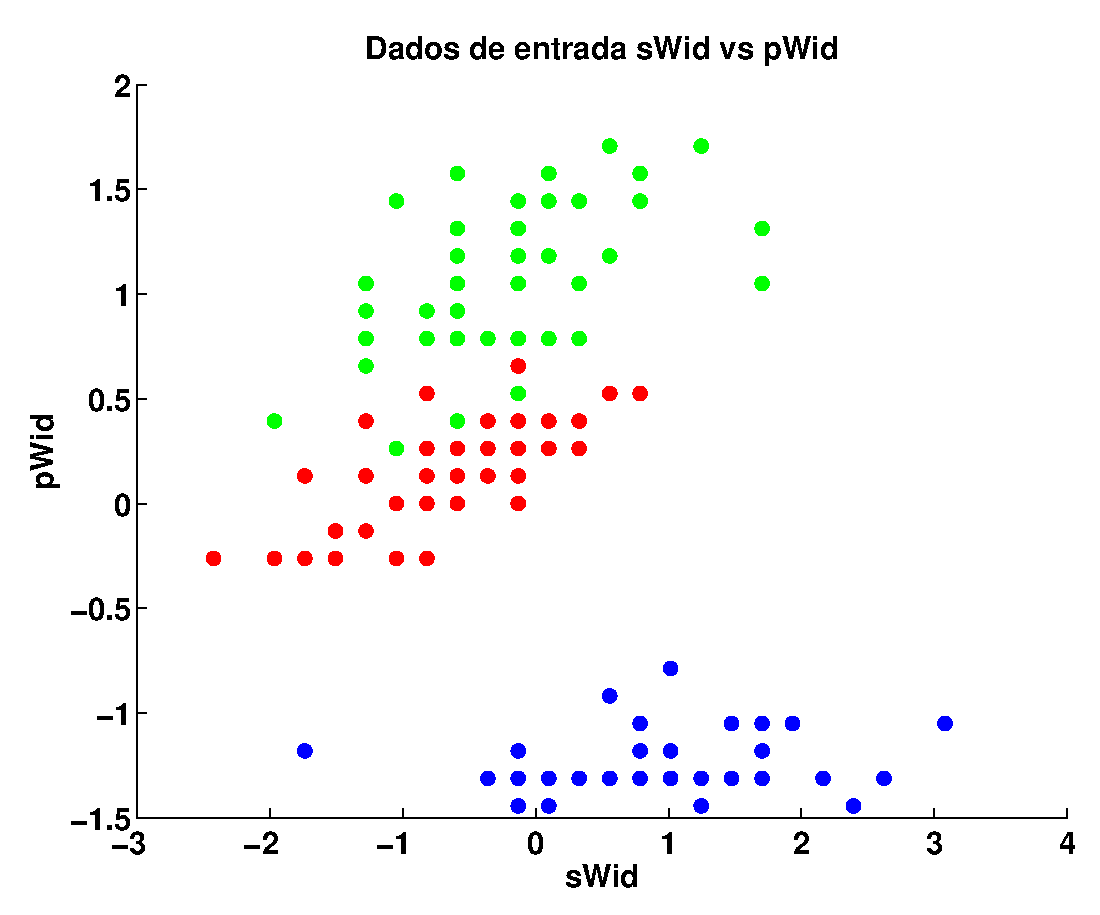
\includegraphics[width=\textwidth]{eps/3classes/input/sWid-vs-pWid.eps}
	\end{subfigure} 
	\begin{subfigure}[h]{0.3\textwidth}
		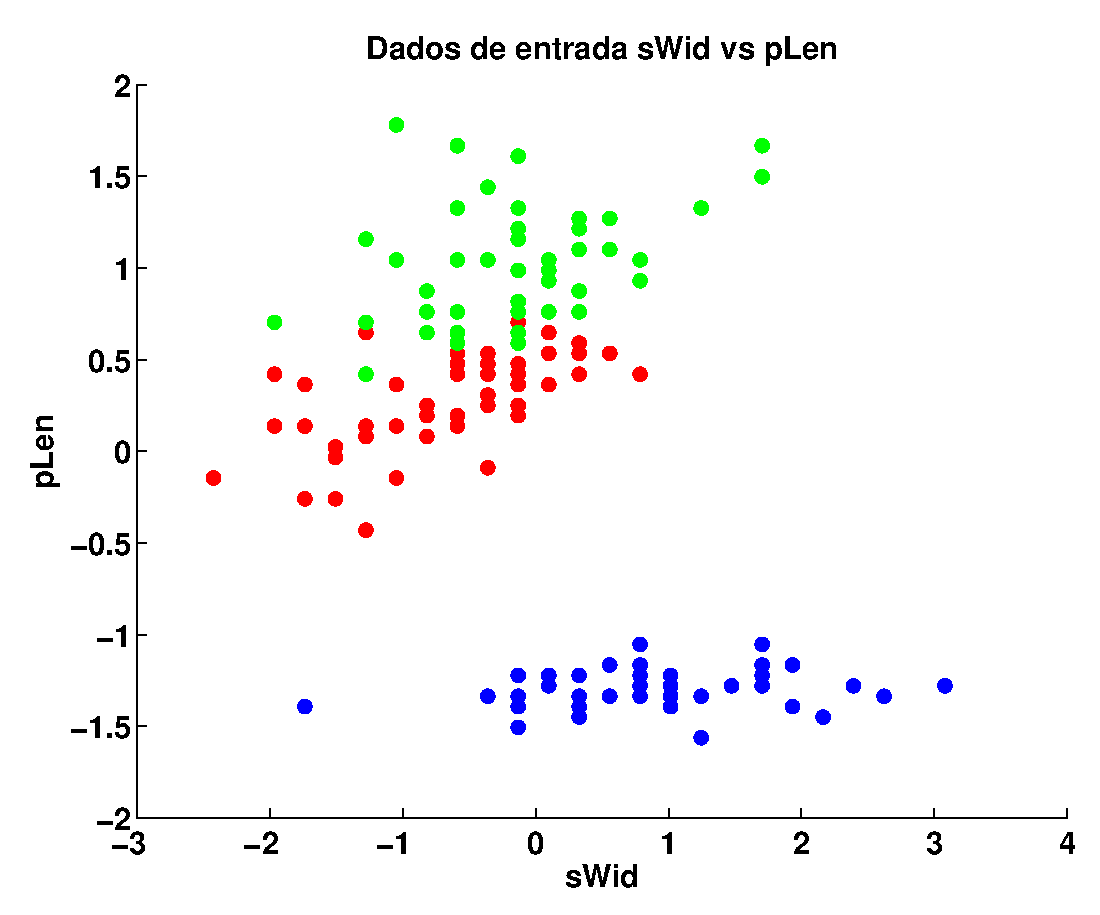
\includegraphics[width=\textwidth]{eps/3classes/input/sWid-vs-pLen.eps}
	\end{subfigure} 
	\caption{Caractéristicas do DataSet da Íris combinados}
\end{figure}


\subsection{Implementação do Perceptron}

Abaixo é possível visualizar o código implementado em Matlab para executar o
treinamento do perceptron. Está função considera que o bias foi previamente
adicionado como se fosse uma característica do dado de entrada.
\lstinputlisting[]
{code/perceptron/perceptron.m}


\subsection{Exemplo de utilização do Perceptron}

Abaixo é possível visualizar o código implementado em Matlab para executar e
avaliar o treinamento do perceptron. 
\lstinputlisting[]
{code/perceptron/testPerceptron.m}
% Can use something like this to put references on a page
% by themselves when using endfloat and the captionsoff option.
\ifCLASSOPTIONcaptionsoff
  \newpage
\fi



% trigger a \newpage just before the given reference
% number - used to balance the columns on the last page
% adjust value as needed - may need to be readjusted if
% the document is modified later
%\IEEEtriggeratref{8}
% The "triggered" command can be changed if desired:
%\IEEEtriggercmd{\enlargethispage{-5in}}

% references section

% can use a bibliography generated by BibTeX as a .bbl file
% BibTeX documentation can be easily obtained at:
% http://www.ctan.org/tex-archive/biblio/bibtex/contrib/doc/
% The IEEEtran BibTeX style support page is at:
% http://www.michaelshell.org/tex/ieeetran/bibtex/
%\bibliographystyle{IEEEtran}
% argument is your BibTeX string definitions and bibliography database(s)
%\bibliography{IEEEabrv,../bib/paper}
%
% <OR> manually copy in the resultant .bbl file
% set second argument of \begin to the number of references
% (used to reserve space for the reference number labels box)
\begin{thebibliography}{1}

\bibitem{IEEEhowto:kopka}
CS 4793: Introduction to Artificial Neural Networks. Department of Computer
Science, University of Texas at San Antonio.

\bibitem{IEEEhowto:kopka}Braga, Antônio de Pádua; Carvalho, André P. L.
Ferreira; Ludermir, Teresa Bernarda, "Redes Neurais Artificiais: Teoria e Aplicações" (2000), Rio de Janeiro: LTC.

\bibitem{IEEEhowto:kopka}
HAYKIN, Simon. Redes neurais: princípios e prática. trad. Paulo Martins Engel. -2.ed. - Porto Alegre: Bookman, 2001.

\bibitem{IEEEhowto:kopka}
http://users.ics.aalto.fi/ahonkela/dippa/node41.html
\bibitem{IEEEhowto:kopka}
http://reference.wolfram.com/applications/neuralnetworks/NeuralNetworkTheory/2.4.0.html
\bibitem{IEEEhowto:kopka}
http://www.gsigma.ufsc.br/~popov/aulas/rna/neuronio\_artificial/index.html

\end{thebibliography}


% biography section
% 
% If you have an EPS/PDF photo (graphicx package needed) extra braces are
% needed around the contents of the optional argument to biography to prevent
% the LaTeX parser from getting confused when it sees the complicated
% \includegraphics command within an optional argument. (You could create
% your own custom macro containing the \includegraphics command to make things
% simpler here.)
%\begin{IEEEbiography}[{\includegraphics[width=1in,height=1.25in,clip,keepaspectratio]{mshell}}]{Michael Shell}
% or if you just want to reserve a space for a photo:

%\begin{IEEEbiography}[{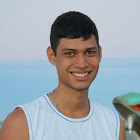
\includegraphics[width=1in,height=1.25in,clip,keepaspectratio]{images/eu.JPG}}]{David
%Clifte}Bacharel em Engenharia de Telecomunicações, IFCE - 2013,\newline
%Mestrando em Ciências da Computação, IFCE
%\end{IEEEbiography}


% You can push biographies down or up by placing
% a \vfill before or after them. The appropriate
% use of \vfill depends on what kind of text is
% on the last page and whether or not the columns
% are being equalized.

%\vfill

% Can be used to pull up biographies so that the bottom of the last one
% is flush with the other column.
%\enlargethispage{-5in}



% that's all folks
\end{document}


